%===============================================================================
% ifacconf.tex 2022-02-11 jpuente  
% 2022-11-11 jpuente change length of abstract
% Template for IFAC meeting papers
% Copyright (c) 2022 International Federation of Automatic Control
%===============================================================================
\documentclass[numbers]{ifacconf}

\usepackage{graphicx}      % include this line if your document contains figures
\graphicspath{ {./figures/} }
\usepackage{adjustbox} % adjust figures on left or right

\makeatletter
\let\old@ssect\@ssect % Store how ifacconf defines \@ssect
\makeatother

\usepackage{amsmath}
\usepackage{amssymb}
\usepackage{mathtools}
\usepackage{enumerate}

\usepackage{enumitem}

%---------- References --------------
\usepackage{hyperref} % Adds clickable links at references
%\usepackage{cleveref}
\usepackage[square, numbers, sort&compress]{natbib} % Square brackets, citing references with numbers, citations sorted by appearance in the text and compressed
\bibliographystyle{abbrvnat} % You may use a different style adapted to your field

\makeatletter
\def\@ssect#1#2#3#4#5#6{%
  \NR@gettitle{#6}% Insert key \nameref title grab
  \old@ssect{#1}{#2}{#3}{#4}{#5}{#6}% Restore ifacconf's \@ssect
}
\makeatother

%===============================================================================

\begin{document}

%===============================================================================

\begin{frontmatter}

% \includegraphics[scale=0.4]{logo_polimi}

\title{The Boundary Element Method: Theoretical Formulation, Numerical Approximation, and Parallel Implementation}

Type A project for the \textit{Numerical Analysis for PDEs} course

\author[first]{Matteo Bonfadini\thanksref{ty}}, 
\author[second]{Manuel Alfano\thanksref{ty}}

\thanks[ty]{We deeply thank for the opportunity Prof. P.F.Antonietti, Dr. F. Regazzoni, Dr. C. B. Leimer Saglio, and for the support Dr. I. Mazzieri.} 

\address[first]{Politecnico di Milano,
Piazza Leonardo da Vinci 32, 20133 Milano, Italy (e-mail: \normalfont\texttt{matteo.bonfadini@mail.polimi.it})}

\address[second]{Politecnico di Milano,
Piazza Leonardo da Vinci 32, 20133 Milano, Italy (e-mail: \normalfont\texttt{manuel.alfano@mail.polimi.it})}

\textit{May 23, 2024}

%!TEX root = ../main.tex

\begin{abstract} % Abstract of 50--100 words
The past fifty years have been marked by the evolution of computers and an enormous availability of computational power. This has boosted the development of computational methods and their application in engineering. The most popular computational method is the Finite Element Method (FEM), however around 1970 the engineering community started to develop the Boundary Element Method (BEM). This work considers the BEM theoretical formulation, and both its numerical approximation and parallel implementation based on the $\pi$-\texttt{BEM} library.
\end{abstract}

\begin{keyword}
BEM \sep 
Fundamental solution \sep
Collocation method \sep
Fast multipole method \sep
MPI
\end{keyword}

\end{frontmatter}

%===============================================================================

%!TEX root = ../main.tex

\section{Introduction}
\label{sec:Introduction}

The term \emph{Boundary Element Method} was coined in 1977 in three publications: Banerjee and Butterfield, Brebbia and Dominguez, and Dominguez. The mathematical foundations were established by Betti in 1872 and Somigliana in 1886 for elasticity problems. Additionally, Green in 1828 and Fredholm in 1903 made foundational contributions to potential problems.

A fair question to ask is "why do we need the BEM since we already have the FEM that solves engineering problems?". The answer is that modeling with finite elements can be ineffective and laborious for certain classes of problems. So the FEM, despite the generality of its application in engineering problems, is not free of drawbacks. The most important advantages of preferring BEM over FEM are:
\begin{enumerate}
  \item The solution is mathematically expressed as a continuous mathematical formula, namely a Boundary Integral Equation (BIE). Therefore the associated numerical method, the BEM, benefits of a discretization only over the boundary $\Gamma$ of the problem domain $\Omega$, leading to a significant reduction in the number of degrees of freedom of the numerical model (see Fig.~\ref{fig:bem-fem-mesh}).

  \begin{figure}
  \begin{center}
    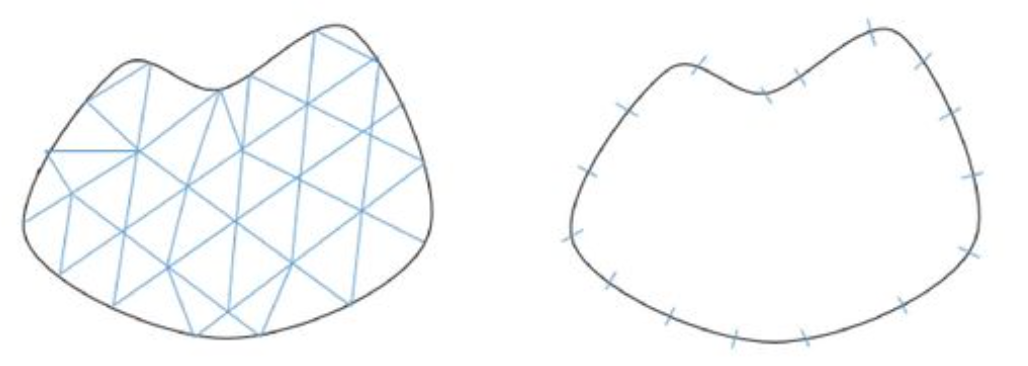
\includegraphics[width=8.4cm]{bem-fem-mesh}    % The printed column width is 8.4 cm.
    \caption{FEM versus BEM domain discretization.} 
    \label{fig:bem-fem-mesh}
  \end{center}
  \end{figure}

  \item The method is particularly effective in computing accurately the derivatives of the field function (e.g., fluxes, strain, stresses, moments).  Instead, in FE methods the accuracy drops considerably in areas of large gradients.

  However, we mention that in mixed Neumann Dirichlet problems with Lipschitz domain there arises an issue when considering continuous elements. A possible solution is the so-called double node technique, where, thanks to the splitting of a physical node into more computational nodes, continuity is preserved only on the solution, while its normal gradient is allowed to have a jump across physical edges.

  \item For infinite domains, the problem is formulated simply as an exterior one. In this manner, computer programs developed for finite domains can be used, with just a few modifications, to solve problems in infinite domains. This is not possible with the FEM.

  \item Even if nowadays there a lot of advanced professional FE softwares equipped with automatic and adaptable mesh generators, the BEM is well suited for solving problems in domains with geometric peculiarities, such as cracks and holes. Moreover, BEM is more feasible for problems described by differential equations of fourth or higher order (e.g., plate equation).
\end{enumerate}

On the other hand, the BEM exhibits the following main disadvantages:
\begin{enumerate}
\setcounter{enumi}{5}
  \item Application of the BEM requires the establishment of the BIE. This is possible only if the problem is linear and its fundamental solution can be established, such as for Laplace equation, Helmholtz equation, and Stokes system. Hence, the method cannot be used for problems whose fundamental solution is either unknown or cannot be determined. Such are, for example, problems described by differential equations with variable coefficients.

  \item The numerical implementation of the BEM results in systems of linear algebraic equations whose coefficient matrices are fully populated and nonsymmetrical. Moreover, if one considers mixed Neumann Dirichlet boundary value problems the final linear system is generally ill conditioned. In a FEM model, however, the corresponding matrices have some very nice properties, they are banded and symmetric. This drawback of the BEM is counterbalanced by a smaller dimension of its matrices (see Fig.~\ref{fig:bem-fem-grid}).

  \begin{figure}
  \begin{centering}
    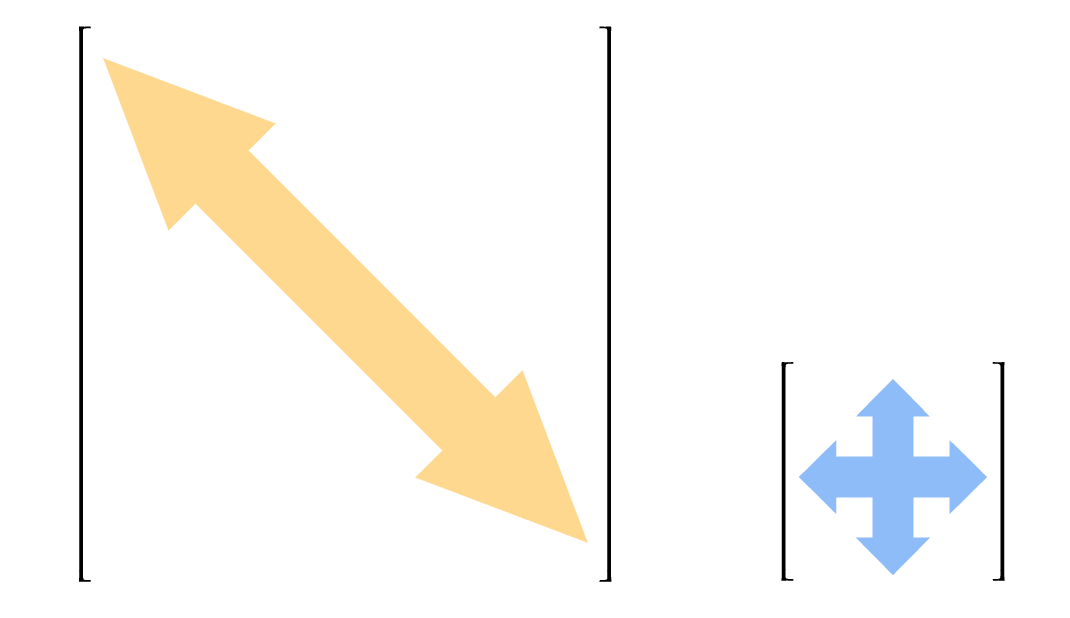
\includegraphics[width=8.4cm]{bem-fem-grid.png}
    \caption{FEM versus BEM coefficient matrix.}
    \label{fig:bem-fem-grid}
  \end{centering}
  \end{figure}
\end{enumerate}

A number of steps are possible to improve the applicability of BEM. We begin by discussing high order elements, which reduce the number of degrees of freedom needed to achieve a certain tolerance in problems with smooth solutions. High order BEMs are more attractive when compared to their FE counterparts, since increasing the order in finite elements leads to a denser, more ill conditioned system matrix. In the case of BEM the matrices, accordingly to drawback (7), are already full, and this is no more a disadvantage. If the solution is non smooth, one can combine high order elements with local refinement techniques to achieve the same result.

As the size of problem increases, none of these techniques alone is enough to reduce memory problems. Then it is usually applied a domain decomposition by exploiting distributed memory techniques, which reduce the number of degree of freedom handled by each processor. Moreover, in order to optimize BEM matrix-vector product operations from $\mathcal{O}(N^2)$ to $\mathcal{O}(N)$ it has been developed the so-called Fast Multipole Method (FMM), which thanks to a hierarcical structure (see Fig.~\ref{fig:hiera}) can decompose short and long range interaction. 

\begin{figure}
  \begin{center}
    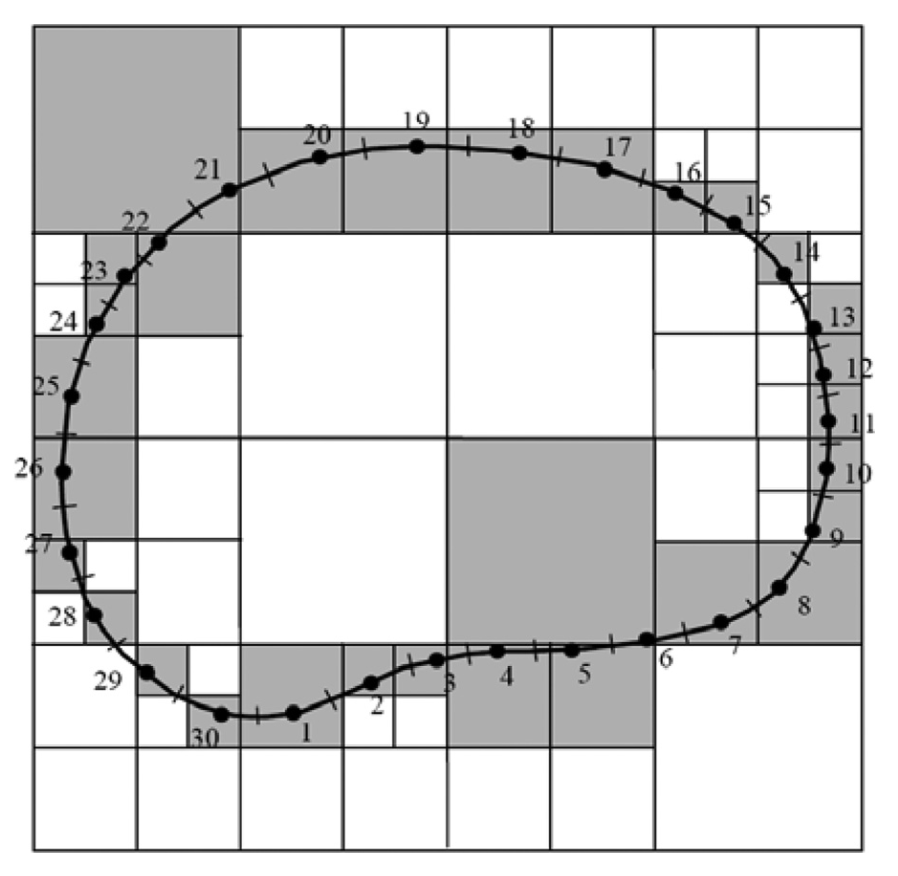
\includegraphics[width=4.2cm]{hiera1} \\
    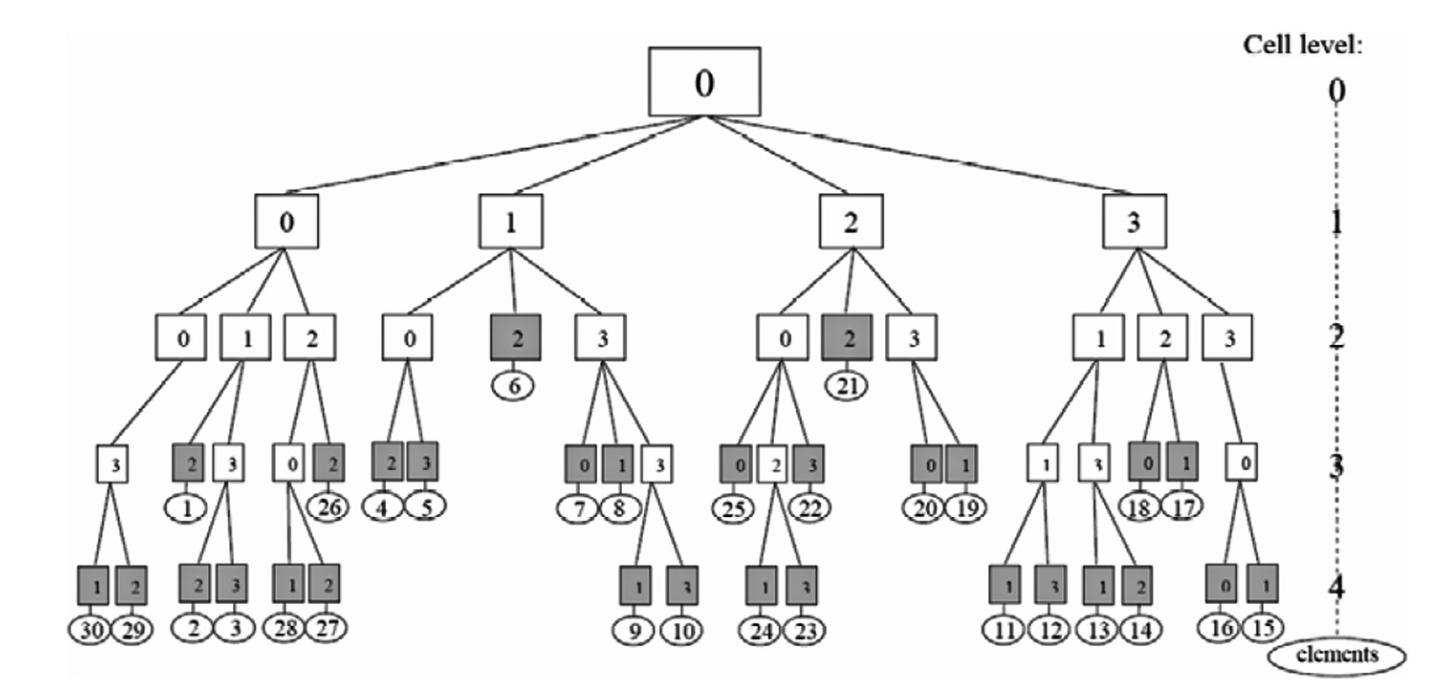
\includegraphics[width=8.4cm]{hiera2}   % The printed column width is 8.4 cm.
    \caption{Hierarchical quad-tree structure for a 2D boundary element mesh.} 
    \label{fig:hiera}
  \end{center}
\end{figure}

Nowadays, boundary integral formulation and in particular the Fast Multipole BEM (FMBEM) have been applied to problems involving hydrodynamic flows (e.g., Fig.~\ref{fig:fish}), flow around aerodynamic lifting bodies, structural mechanics, electrostatics, quantum mechanics, and acoustics (e.g., Fig.~\ref{fig:skipjack}-\ref{fig:dummy-head}). See~\ref{Katsi},\ref{Attilio} for more delailed explanations. 

\begin{figure}
  \begin{center}
    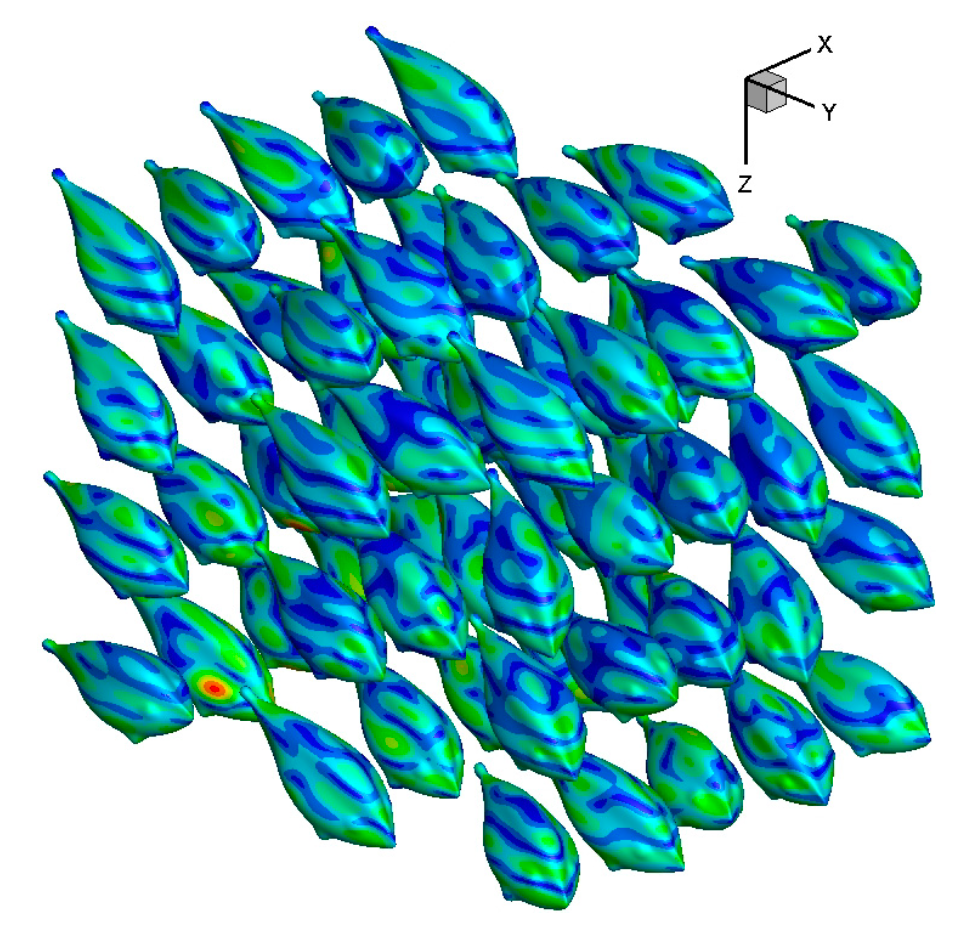
\includegraphics[width=5.6cm]{fish}    % The printed column width is 8.4 cm.
    \caption{Scattering of a multiple fish model.} 
    \label{fig:fish}
  \end{center}
\end{figure}

\begin{figure}
  \begin{center}
    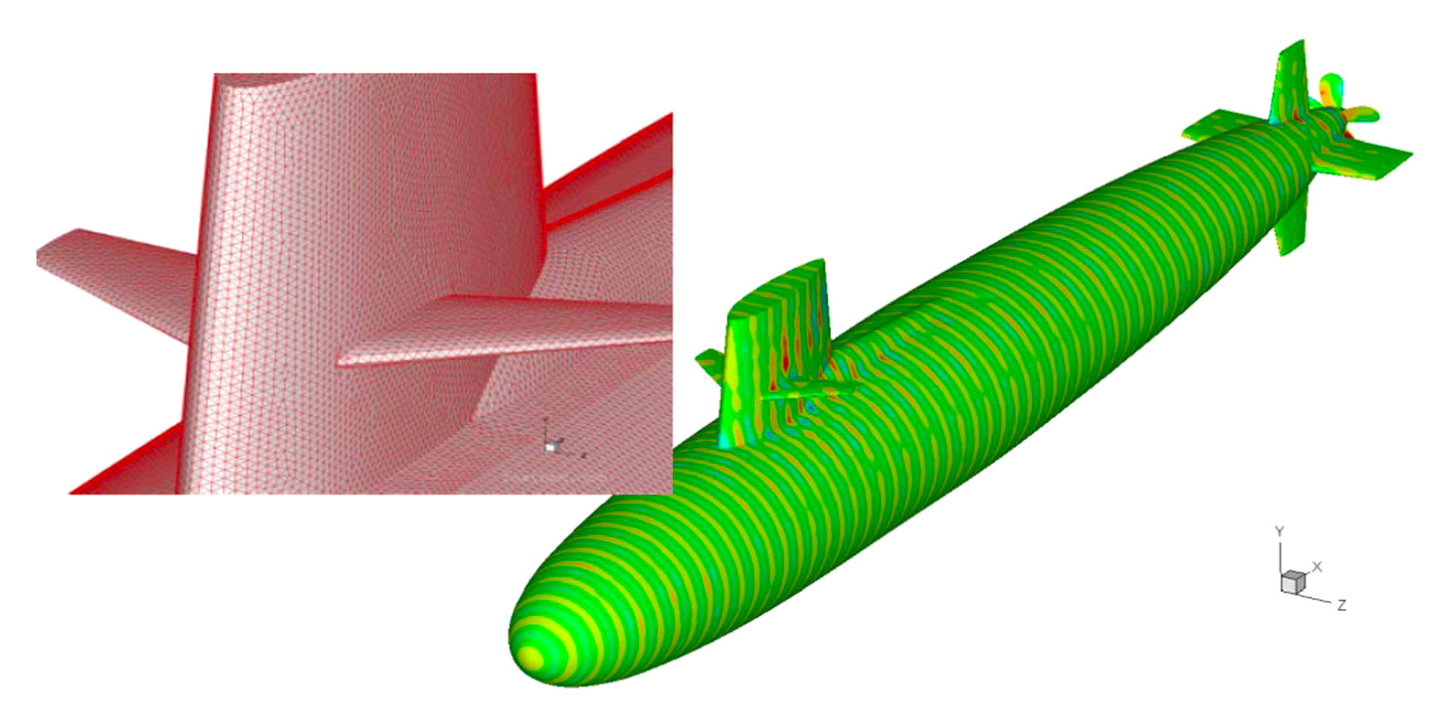
\includegraphics[width=8.4cm]{skipjack}    % The printed column width is 8.4 cm.
    \caption{BEM model of the Skipjack submarine impinged upon by an incident wave in the direction $(1, 0, \text{-}1)$.} 
    \label{fig:skipjack}
  \end{center}
\end{figure}

\begin{figure}
  \begin{center}
    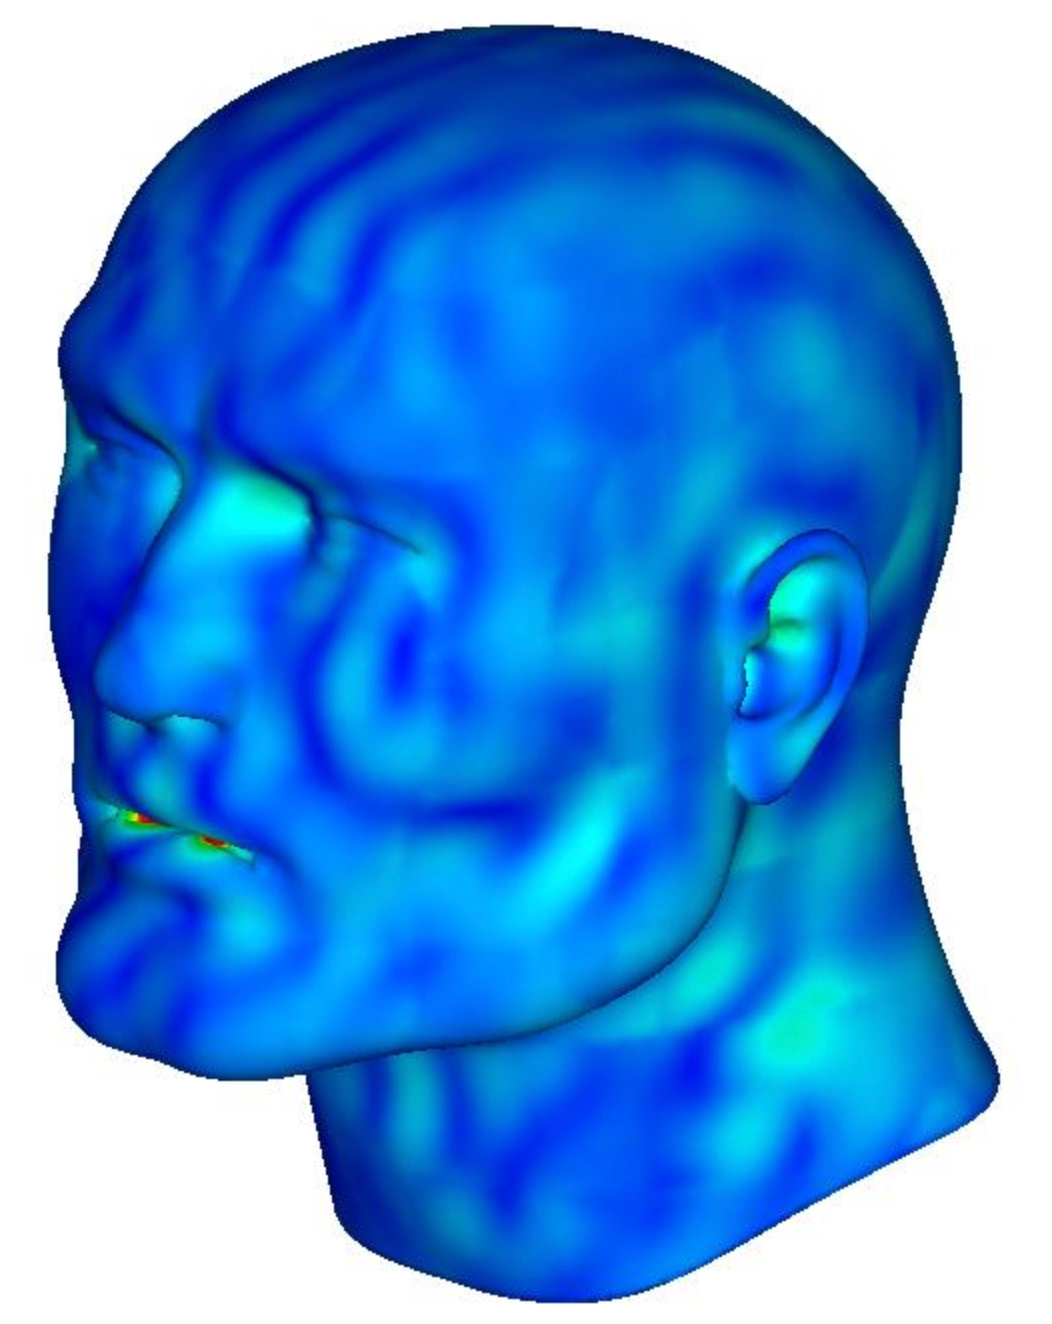
\includegraphics[width=4.2cm]{dummy-head}    % The printed column width is 8.4 cm.
    \caption{BEM mesh and sound-pressure plots for a human-head model.} 
    \label{fig:dummy-head}
  \end{center}
\end{figure}

In ths work, we are going to present for a model Laplace problem the theoretical background of BEM methodologies, as well as convergence and scalability tests of the parallel implementation carried out in \ref{Mola}.








%!TEX root = ../main.tex

\section{Boundary Integral Formulation}
\label{sec:BoundaryIntegralFormulation}

We consider a bounded open domain $\Omega\subseteq\mathbb{R}^3$ with Lipschitz boundary $\Gamma=\partial\Omega$, and we want to solve potential problems described by the Laplace equation
\begin{equation}
\label{eq:poisson-eq}
\Delta \phi=0\qquad \text{ in }\Omega.
\end{equation}

We couple Eq.~\eqref{eq:poisson-eq} with the following boundary conditions:
\begin{subequations}
\label{eq:BCs}
\begin{align}
\label{eq:Dirichlet}
\phi=f_D &\qquad \text{ on }\Gamma_D, \\
\label{eq:Neumann} 
\frac{\partial\phi}{\partial n}=f_N &\qquad \text{ on }\Gamma_N, 
\end{align}
\end{subequations}

where $\frac{\partial \phi}{\partial n}=\nabla \phi\cdot \mathbf{n}$, $\Gamma_D\cup\Gamma_N=\Gamma$, $\Gamma_D\cap\Gamma_N=\varnothing$, and $\Gamma_D\neq\varnothing$.

\subsection{Laplace Equation in Distributional Form}
\label{sub:lapDistrib}%

Before dealing with Eq.~\eqref{eq:poisson-eq}, let us consider the following equation:
\begin{equation}
\label{eq:fundamental-eq}
-\Delta \phi(\mathbf{y})=\delta_\mathbf{x}\qquad\forall\,\mathbf{y}\in\mathbb{R}^3.
\end{equation}

This is known as the Poisson equation in the whole space. Here, $\phi(\mathbf{y})$ represents the potential produced at a point $\mathbf{y}$ in the domain $\Omega$ generated by a unit point source placed at point $\mathbf{x}$, i.e., the Dirac Delta function $\delta_\mathbf{x}$. A solution of Eq.~\eqref{eq:fundamental-eq} is called the fundamental solution of the laplacian, and it can be determined as follows.

We write Eq.~\eqref{eq:fundamental-eq} in polar coordinates with origin at $\mathbf{x}$. Since this solution is axisymmetric with respect to the source, it is independent of the polar angle $\theta$, thus the three-dimensional laplacian is
\begin{equation*}
\Delta \phi = \phi_{rr} + \frac{2}{r}\ \phi_r,
\end{equation*}

where $r=\left| \mathbf{x}-\mathbf{y} \right|$ is the Euclidean distance between $\mathbf{x}$ and $\mathbf{y}$. The right-hand side vanishes at all points of the plane, except at the origin $r=0$ (or $\mathbf{y}=\mathbf{x}$), where it has infinite value. Then Eq.~\eqref{eq:fundamental-eq} is written as
\begin{equation*}
\phi_{rr} + \frac{2}{r}\ \phi_r = 0 \qquad \forall\, r>0.
\end{equation*}

The change of variables $\phi_r=v$ gives us 
\begin{equation*}
\begin{gathered}
v' + \frac{2}{r}\ v = 0 \quad \leadsto \quad \int \frac{v'}{v}= \int -\frac{2}{r}  \\ \leadsto \quad \log(v) =-2\log(r)+c \quad \leadsto \quad v=\frac{c}{r^2}  ,  
\end{gathered}
\end{equation*}

then 
\begin{equation*}
\phi=\int \frac{c}{r^2} = \frac{c_1}{r} +c_2.
\end{equation*}

Since we want a particular solution we may set $c_2=0$, and to determine $c_1$ we perform an integration by parts on Eq.~\eqref{eq:fundamental-eq} over a ficticious unit circular domain $\Omega$:
\begin{equation*}
\int_\Omega -\Delta \phi\ \varphi \ \mathrm{d}\Omega = -\int_{\partial\Omega}\frac{\partial \phi}{\partial n}\ \varphi \ \mathrm{d}S+\int_\Omega \nabla \phi \cdot \nabla \varphi \ \mathrm{d}\Omega
\end{equation*}

which, for $\varphi\equiv 1$, reads
\begin{equation*}
\int_\Omega \delta_\mathbf{x}\ \mathrm{d}\Omega = \int_{\partial\Omega}\frac{\partial \phi}{\partial n} \ \mathrm{d}S.
\end{equation*}

Due to the axisymmetric nature of the problem
\begin{equation*}
\frac{\partial \phi}{\partial n}=\frac{\partial \phi}{\partial r} = \frac{c_1}{r^2}
\end{equation*}
thus, after using the definition of Delta function and performing an integration in radial coordinates, we are left with
\begin{equation*}
1=4\pi \int_0^1 \rho^2\ v(\rho) \ \mathrm{d}\rho = 4\pi \int_0^1 \rho^2\ \frac{c_1}{\rho^2} \ \mathrm{d}\rho =4\pi c_1.
\end{equation*}

We discovered $c_1=\frac{1}{4\pi}$, hence, the fundamental solution becomes $\phi=\frac{1}{4\pi r}$, which is also known in the literature as the free space Green's function:
\begin{equation}
\label{eq:green-fun}
G(\mathbf{x},\mathbf{y})=\frac{1}{4\pi \left| \mathbf{x}-\mathbf{y} \right|}\qquad \forall\,\mathbf{y}\in\mathbb{R}^3.
\end{equation}

One can easily prove (see for example \ref{Evans}) that this expression is the solution of $-\Delta G(\mathbf{x},\cdot)=\delta_\mathbf{x}$ in $\mathcal{D}'(\mathbb{R}^3)$, i.e., in the distributional sense. 

\subsection{BEM for the Laplace Equation}
\label{sub:bem_for_the_laplace_equation}

Here we derive the solution of the Laplace equation~\eqref{eq:poisson-eq} with mixed boundary conditions~\eqref{eq:BCs}. 

We can multiply the Laplace equation by an arbitrary test function $\varphi$ and integrate by parts twice:
\begin{gather*}
0=\int_\Omega -\Delta \phi\ \varphi \ \mathrm{d}\Omega = - \int_{\Gamma} \frac{\partial \phi}{\partial n}\ \varphi \ \mathrm{d}S + \int_\Omega \nabla \phi\ \nabla \varphi\ \mathrm{d}\Omega \\ 
= - \int_{\Gamma} \frac{\partial \phi}{\partial n}\ \varphi \ \mathrm{d}S + \int_{\Gamma} \frac{\partial \varphi}{\partial n}\ \phi \ \mathrm{d}S - \int_\Omega \Delta \varphi\ \phi\ \mathrm{d}\Omega
\end{gather*}

(one could directly apply the Green's second identity). Choosing $\varphi\equiv G$, the free space Green's function defined in Eq.~\eqref{eq:green-fun}, Laplace Eq.~\eqref{eq:poisson-eq} becomes
\begin{equation*}
\int_\Omega -\Delta G\ \phi(\mathbf{y})\ \mathrm{d}\Omega(\mathbf{y}) = \int_{\Gamma} \left[ \frac{\partial \phi}{\partial n}(\mathbf{y})\ G - \frac{\partial G}{\partial n}\ \phi(\mathbf{y}) \right]\!\! \ \mathrm{d}S(\mathbf{y}).
\end{equation*}

Since we know that $-\Delta G(\mathbf{x},\mathbf{y})=\delta_\mathbf{x}$,
\begin{equation*}
\int_\Omega \delta_\mathbf{x}\ \phi(\mathbf{y})\ \mathrm{d}\Omega(\mathbf{y}) = \int_{\Gamma} \left[ \frac{\partial \phi}{\partial n}(\mathbf{y})\ G- \frac{\partial G}{\partial n}\ \phi(\mathbf{y}) \right]\!\! \ \mathrm{d}S(\mathbf{y})
\end{equation*}

hence, by the definition of Dirac Delta, we are left with
\begin{equation}
\label{eq:integral-rep}
\phi(\mathbf{x}) = \int_{\Gamma} \left[ \frac{\partial \phi}{\partial n}(\mathbf{y})\ G(\mathbf{x},\mathbf{y}) - \frac{\partial G}{\partial n}(\mathbf{x},\mathbf{y})\ \phi(\mathbf{y}) \right]\!\! \ \mathrm{d}S(\mathbf{y})
\end{equation}

$\forall\, \mathbf{x} \in\Omega$. This expression is the integral representation of the solution for the Laplace equation at any point $\mathbf{x}$ inside the domain $\Omega$ in terms of the boundary values of $\phi$ and its normal derivative ${\partial \phi}/{\partial n}$. It is apparent from the boundary conditions~\eqref{eq:Dirichlet} and~\eqref{eq:Neumann}, that only one of the quantities $\phi$ or $\partial\phi/\partial n$ is prescribed at a point $\mathbf{y}$ on the boundary.  Consequently, it is not yet possible to determine the solution from the integral representation~\eqref{eq:integral-rep}. Therefore, we let $\mathbf{x}$ lie on the boundary $\Gamma$: we notiche that the kernels $G(\mathbf{x},\mathbf{y})$ and $\frac{\partial G}{\partial n}(\mathbf{x},\mathbf{y})$ become weakly singular (but integrable) and singular respectively. Hence, considering the Cauchy Principal Value (CPV) of the $\frac{\partial G}{\partial n}$ singular integral, we can write
\begin{equation}
\label{eq:solid-angle}
\resizebox{.9\hsize}{!}{
$\alpha(\mathbf{x})\phi(\mathbf{x}) = \displaystyle\int_{\Gamma} \frac{\partial \phi}{\partial n}(\mathbf{y})\ G(\mathbf{x},\mathbf{y})\ \mathrm{d}S(\mathbf{y}) - \int_{\Gamma}^{\text{PV}} \frac{\partial G}{\partial n}(\mathbf{x},\mathbf{y})\ \phi(\mathbf{y}) \ \mathrm{d}S(\mathbf{y}),$}
\end{equation}

where the coefficient $\alpha(\mathbf{x})$ is obtained fromt the CPV evaluation of the singular integral, and it represents the fraction of solid angle (see Fig.~\ref{fig:angle}) with which the domain $\Omega$ is seen from the boundary point $\mathbf{x}$:
\begin{equation*}
\alpha(\mathbf{x})=
\begin{cases}
1 &\text{ for } \mathbf{x} \text{ inside } \Omega, \\ 
\textstyle\frac{\theta_1-\theta_2}{2\pi} &\text{ for } \mathbf{x} \text{ on the boundary } \Gamma, \\
0 &\text{ for } \mathbf{x} \text{ outside } \Omega.
\end{cases}
\end{equation*}

In particular, $\alpha=1/2$ for smooth boundary points.

\begin{figure}
  \begin{center}
    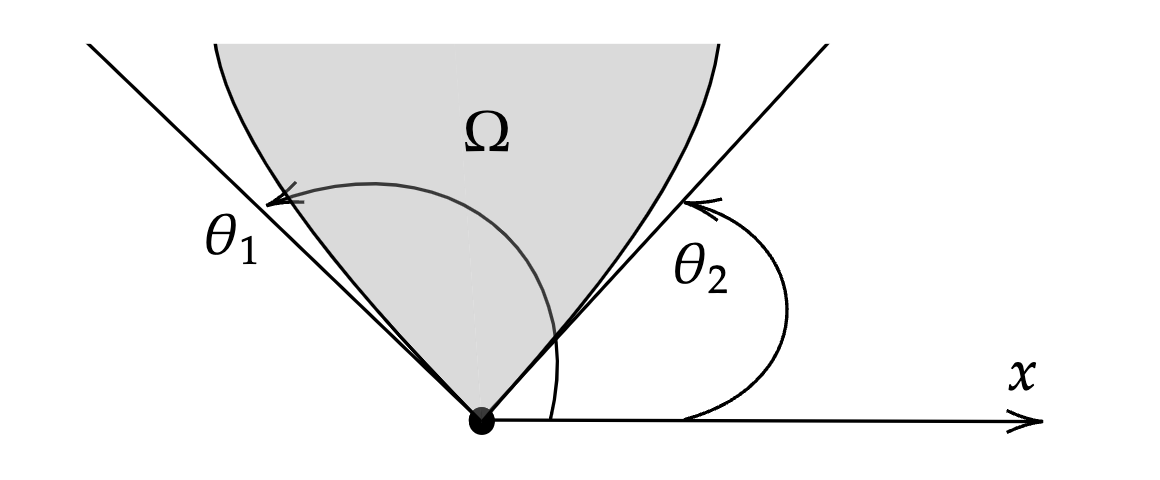
\includegraphics[width=8.4cm]{angle}    % The printed column width is 8.4 cm.
    \caption{Solid angle related to a corner point of a nonsmooth boundary.} 
    \label{fig:angle}
  \end{center}
\end{figure}

By explicitly writing the boundary conditions using the characteristic function $\chi_{_A}(\mathbf{x})$, which is one if $\mathbf{x}\in A$ and zero otherwise, we obtain
\begin{equation*}
\begin{gathered}
\resizebox{.9\hsize}{!}{
$\chi_{_{\Gamma_{\!N}}}\!(\mathbf{x})\alpha(\mathbf{x})\phi(\mathbf{x}) - \displaystyle\int_{\Gamma_{\!N}} f_{_N}(\mathbf{y})\ G(\mathbf{x},\mathbf{y})\ \mathrm{d}S(\mathbf{y}) + \int_{\Gamma_{\!N}}^{\text{PV}} \frac{\partial G}{\partial n}(\mathbf{x},\mathbf{y})\ \phi(\mathbf{y}) \ \mathrm{d}S(\mathbf{y})=$} \\
\resizebox{.9\hsize}{!}{
$= - \chi_{_{\Gamma_{\!D}}}\!(\mathbf{x})\alpha(\mathbf{x})f_{_D}(\mathbf{x}) + \displaystyle\int_{\Gamma_{\!D}} \frac{\partial\phi}{\partial n}(\mathbf{y})\ G(\mathbf{x},\mathbf{y})\ \mathrm{d}S(\mathbf{y}) - \int_{\Gamma_{\!D}}^{\text{PV}} \frac{\partial G}{\partial n}(\mathbf{x},\mathbf{y})\ f_{_D}(\mathbf{y}) \ \mathrm{d}S(\mathbf{y}).$}
\end{gathered}
\end{equation*}

Grouping all the unknowns in the left-hand side we finally deduce
\begin{equation}
\label{eq:characteristic-angle}
\begin{gathered}
\resizebox{.9\hsize}{!}{
$\chi_{_{\Gamma_{\!N}}}\!(\mathbf{x})\alpha(\mathbf{x})\phi(\mathbf{x}) - \displaystyle\int_{\Gamma_{\!D}} \frac{\partial \phi}{\partial n}(\mathbf{y})\ G(\mathbf{x},\mathbf{y})\ \mathrm{d}S(\mathbf{y}) + \int_{\Gamma_{\!N}}^{\text{PV}} \frac{\partial G}{\partial n}(\mathbf{x},\mathbf{y})\ \phi(\mathbf{y}) \ \mathrm{d}S(\mathbf{y})=$} \\
\resizebox{.9\hsize}{!}{
$= - \chi_{_{\Gamma_{\!D}}}\!(\mathbf{x})\alpha(\mathbf{x})f_{_D}(\mathbf{x}) + \displaystyle\int_{\Gamma_{\!N}} f_{_N}(\mathbf{y})\ G(\mathbf{x},\mathbf{y})\ \mathrm{d}S(\mathbf{y}) - \int_{\Gamma_{\!D}}^{\text{PV}} \frac{\partial G}{\partial n}(\mathbf{x},\mathbf{y})\ f_{_D}(\mathbf{y}) \ \mathrm{d}S(\mathbf{y}).$}
\end{gathered}
\end{equation}

Eq.~\eqref{eq:characteristic-angle} simply is the trace of Eq.~\eqref{eq:integral-rep}, namely it is the BIE with which it is possible to derive the potential where its normal derivative is known, and viceversa.









%!TEX root = ../main.tex

\section{Discretisation}
\label{sec:Discretisation}

We use standard Lagrangian finite element spaces on $\Gamma$ as basis functions both for the geometry and the unknowns $\phi$ and $\frac{\partial\phi}{\partial n}=:\gamma$. The approximation can be divided in 6 main steps.

\subsection{Computational Mesh Generation}
\label{sub:computational_mesh_generation}

We define a quadrilateral computational mesh meant as a regular\footnote{For every cell $K$ there exist a mapping from a reference cell $\hat{K}$ to $K$ with positive determinant of the Jacobian.} decomposition $\Gamma_h$ of the boundary $\Gamma$. Then we progressively refine this very coarse mesh, by exploiting a proper \emph{a posteriori} error estimator, to obtain a solution with desired accuracy.

\subsection{Definition of the Discrete Spaces}
\label{sub:definition_of_the_discrete_spaces}

The right spaces to analyse Eq.~\eqref{eq:solid-angle} are
\begin{equation*}
\phi\in V=H^{1/2}(\Gamma)\qquad \gamma\in Q=H^{-1/2}(\Gamma)
\end{equation*}

In a conforming setting we choose $V_h\subseteq V,\ Q_h\subseteq Q$ as
\begin{subequations}
\label{eq:FEspaces}
\begin{align}
\label{eq:Vhspace}
V_h&:=\left\{ \phi_h\in L^2(\Gamma_h)\,:\,\phi_h\big|_K\in \mathbb{Q}^r(K),\ K\in\Gamma_h \right\}, \\
\label{eq:Qhspace} 
Q_h&:=\left\{ \gamma_h\in L^2(\Gamma_h)\,:\,\gamma_h\big|_K\in \mathbb{Q}^s(K),\ K\in\Gamma_h \right\}.
\end{align}
\end{subequations}


It can be shown that using the same FE discretization for both unknowns does not lead to big disadvantages, thus
\begin{equation*}
V_h=Q_h\equiv \text{span}\{\psi_i\}_{i=1}^{N_V}.
\end{equation*}

\subsection{Collocation of the BIE}
\label{sub:collocation_of_the_bie}

Two approaches are possible in order to discretize Eq.~\eqref{eq:characteristic-angle}. The \emph{Galerkin BEM} is a natural choice and it consists in writing the problem in variational form; however, this implies a second integration of weakly singular kernels, which would increase the computational complexity of the BEM. Therefore, we focus on \emph{collocation methods}. The idea is to directly use the discretized $\phi_h$ and $\gamma_h$ instead of the continuous $\phi$ and $\gamma$, and to collocate the BIE on a number of points equal to the number of unknowns, for example on the support of the Lagrangian basis functions.

We collocate Eq.~\eqref{eq:solid-angle}\footnote{It's simpler to impose the boundary conditions after assembling the linear system.} on the nodes $x_i$ of the boundary mesh, obtaining
\begin{align*}
\alpha(x_i)\phi(x_i)=&\sum_{K\in\Gamma_h}\int_K \gamma(y)\ G(x_i,y)\ \mathrm{d}S(y)\ + \\
& - \sum_{K\in\Gamma_h}\int_K \frac{\partial G}{\partial n}(x_i,y)\ \phi(y)\ \mathrm{d}S(y)
\end{align*}
for every $i=1,\dots,N_V$. Then by a quadrature formula which exploit the geometry of the boundary instead of using generic quadrature weights we get
\begin{align*}
\alpha(x_i)\phi(x_i)=&\sum_{K\in\Gamma_h}\sum_{q=1}^{N_q} \gamma(x_q) G(x_i,x_q) J^K(x_q)\ + \\
& - \sum_{K\in\Gamma_h}\sum_{q=1}^{N_q} \frac{\partial G}{\partial n}(x_i,x_q) \phi(x_q) J^K(x_q),
\end{align*}

where $J^K$ is the determinant of the first fundamental form for each reference cell $\hat{K}$. Now, as we anticipated before, we substitute $\phi$ with its approximation, i.e. $\phi(x_q)\approx \phi_h= \sum_j \phi_j \psi_j(x_q)$. We do the same thing for the flux $\frac{\partial\phi}{\partial n}$, and this yields
\begin{align*}
\alpha(x_i)\phi_j\psi_j(x_i)=&\sum_{K\in\Gamma_h}\sum_{q=1}^{N_q} \gamma_j \psi_j(x_q) G(x_i,x_q) J^K(x_q)\ + \\
& - \sum_{K\in\Gamma_h}\sum_{q=1}^{N_q} \frac{\partial G}{\partial n}(x_i,x_q) \phi_j \psi_j(x_q) J^K(x_q),
\end{align*}

and finally we obtain the linear system
\begin{equation}
\label{eq:first-LS}
(\alpha+N)\hat{\phi}-D\hat{\gamma}=0,
\end{equation}

where
\begin{itemize}
\item $\alpha$ is the diagonal matrix of values $\alpha(x_i)$;
\item $D_{ij}=\sum_K \sum_q G(x_i,x_q)\psi_j^q J^K$;
\item $N_{ij}=\sum_K \sum_q \frac{\partial G}{\partial n}(x_i,x_q)\psi_j^q J^K$;
\item $\hat{\phi}$, $\hat{\gamma}$ are the nodal values of the unknowns.
\end{itemize}

\subsection{Imposition of the Boundary Conditions}
\label{sub:imposition_of_the_boundary_conditions}

To impose the boundary condition for $\phi_h$ and $\gamma_h$, we define the additional vectors
\begin{subequations}
\label{eq:bc-LS}
\begin{align}
\label{eq:bc-LS1}
\tilde{\phi} &= 
\begin{cases}
0 & \text{on } \Gamma_D \\
\hat{\phi} & \text{on } \Gamma_N
\end{cases} \qquad &&
\tilde{\gamma} = 
\begin{cases}
\hat{\gamma} & \text{on } \Gamma_D \\
0 & \text{on }  \Gamma_N
\end{cases} \\
\label{eq:bc-LS2}
\bar{\phi} &= 
\begin{cases}
f_D & \text{on }  \Gamma_D \\
0 & \text{on }  \Gamma_N
\end{cases} \qquad &&
\bar{\gamma} = 
\begin{cases}
0 & \text{on }  \Gamma_D \\
f_N & \text{on } \Gamma_N
\end{cases}
\end{align}
\end{subequations}

With these defintions we can decouple the action of the two unknowns: while \eqref{eq:bc-LS1} clarify the real unknowns, \eqref{eq:bc-LS2} help setting the known values. The decoupled system is 
\begin{equation*}
\begin{cases}
(\alpha+N)\hat{\phi}-D\hat{\gamma}=0 & \text{on }\Gamma_D \\
(\alpha+N)\hat{\phi}-D\hat{\gamma}=0 & \text{on }\Gamma_N
\end{cases}
\end{equation*}
therefore
\begin{equation}
\label{eq:final-LS-with-underbracket}
\underbracket[0.5pt]{(\alpha+N)\tilde{\phi}-D\tilde{\gamma}}_{A\tilde{t}}=\underbracket[0.5pt]{-(\alpha+N)\bar{\phi}+D\bar{\gamma}}_{b}.
\end{equation}

To wrap up, we obtained the linear system $A\tilde{t}=b$, where $\tilde{t}$ simply groups the unknowns:
\begin{equation*}
\tilde{t}_i=
\begin{cases}
\hat{\gamma}_i &\text{if }x_i\in\Gamma_D \\
\hat{\phi}_i &\text{if }x_i\in\Gamma_N  
\end{cases}
\end{equation*}

Notice that the system in Eq.~\eqref{eq:final-LS-with-underbracket} is \emph{one to one} with Eq.~\eqref{eq:characteristic-angle}, as one would expect.

\subsection{Solution of the Linear System}
\label{sub:solution_of_the_linear_system}

In order to solve system \eqref{eq:final-LS-with-underbracket}, we don't assemble the matrix $A$ but we use the Generalized Minimal Residuals (GMRES), which is an iterative method based on Krylov subspace methods. By using least squares (and a preconditioner to accelerate the convergence), we minimize the residual $r^{(k)}=b-At^{(k)}$ till desired accuracy. This procedure works well in BEM frameworks, because it allows you to deal with nonsymmetric and fully populated matrices, and without explicitly forming them, saving a lot of memory.

\subsection{Post Process}
\label{sub:post_process}

We compute an error analysis to verify the proper convergence of the method and if necessary we proceed with a local refinement; then we recover the normal derivative $\frac{\partial \phi}{\partial n}$ (or simply the gradient $\nabla\phi$) by computing the derivative over Eq.~\eqref{eq:solid-angle}, and finally we output the solution.





%!TEX root = ../main.tex

\section{Results}
\label{sec:Results}

We analyse the convergence of the numerical scheme to a known analytical solution 
\begin{equation}
\label{eq:analytical-sol-known}
\phi(x,y,z)=\frac{-1}{4\pi\sqrt{(x-1)^2+(y-0.5)^2+(z-0.5)^2}} 
\end{equation}

for a mixed Dirichlet-Neumann problem on the domain configurations illustrated in Fig.~\ref{fig:original-2} and Fig.~\ref{fig:original-6}.

The first test case considers a sphere of radius $R=1$ and centered in $O=(0,0,0)$. On the left of Fig.~\ref{fig:original-2} we show the initial grid, represented by a simple cube. Dirichlet boundary conditions are applied to the red faces, while Neumann boundary conditions are applied to the blue faces. The right image represents the mesh obtained after 3 global refinement cycles. The possibility to introduce a very coarse initial discretisation of the domain is a key feature of the $\pi$\texttt{-BEM} library.

\begin{figure}[htp]
\begin{center}
    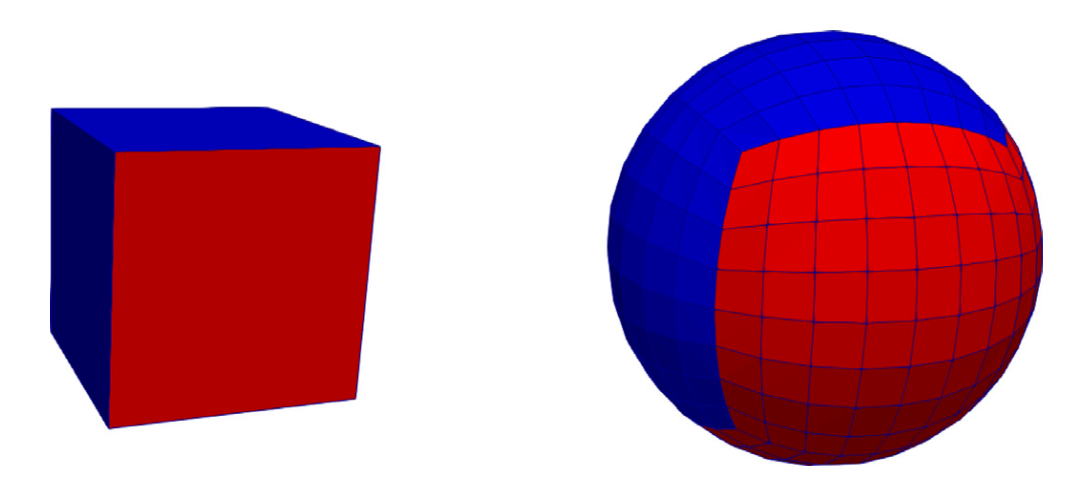
\includegraphics[width=8.4cm]{original-2}    % The printed column width is 8.4 cm.
    \caption{Mesh configuration for the sphere test case with mixed boundary conditions.} 
    \label{fig:original-2}
\end{center}
\end{figure}

While Fig.~\ref{fig:original-3} shows the computed solution $\phi$ over $98304$ cells, Fig.~\ref{fig:original-4} presents the convergence analysis for both the potential (on the left) and its normal derivative (on the right). We obtained a first order convergence on $\phi$ using $Q_1$ elements for both $L_2$ and $L_\infty$ norm. 

\begin{figure}[htp]
\begin{center}
    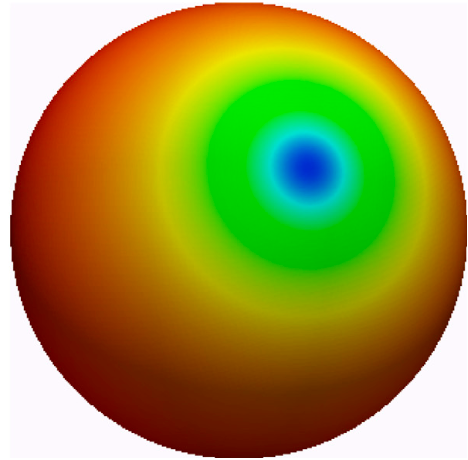
\includegraphics[width=4.2cm]{original-3}    % The printed column width is 8.4 cm.
    \caption{Sphere test case. The colours represent the magnitude of the exact solution $\phi$.} 
    \label{fig:original-3}
\end{center}
\end{figure}

\begin{figure*}[htp]
\begin{center}
    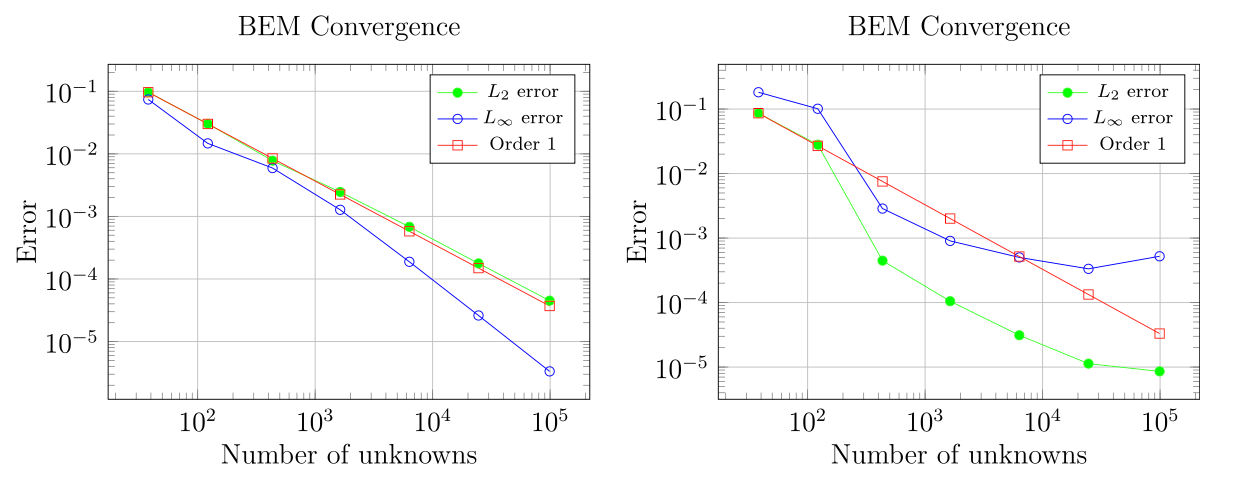
\includegraphics[width=14cm]{original-4}    % The printed column width is 8.4 cm.
    \caption{Convergence analysis for the error in a mixed Dirichlet-Neumann problem using $Q_1$ boundary elements and the spherical mesh. On the left we plot the analysis for the variable $\phi$, on the right we depict the errors for $\frac{\partial\phi}{\partial n}$.} 
    \label{fig:original-4}
\end{center}
\end{figure*}

\newpage

For the normal derivative, we observe a more irregular behavior: initial superconvergence (greater than linear) followed by a significant decrease during the final refinement step. A closer look at the error distribution (see Fig.~\ref{fig:original-5}) suggests that the progressive refinement of an initially cubic mesh over a sphere results in the presence of few stretched cells located at the original mesh vertices. To make things worse such nodes are located at the interface between different boundary condition regions. This situation is not improved throughout the refinements of the grid, as the angle of such stretched cells remain constant for each mesh, which results in a constant error.

\begin{figure}[htp]
\begin{center}
    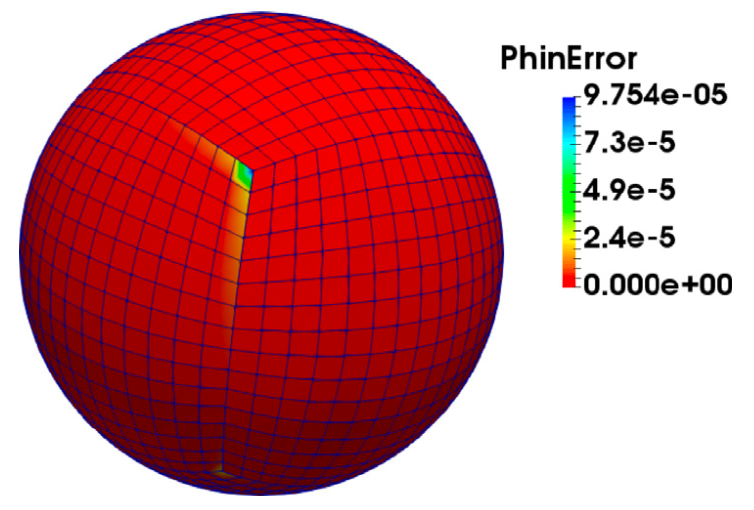
\includegraphics[width=5cm]{original-5}    % The printed column width is 8.4 cm.
    \caption{Error analysis for the potential normal derivative in the sphere test case.} 
    \label{fig:original-5}
\end{center}
\end{figure}

The second test case takes into account the truncated pyramid illustrated in Fig.~\ref{fig:original-6}.

\begin{figure}[htp]
\begin{center}
    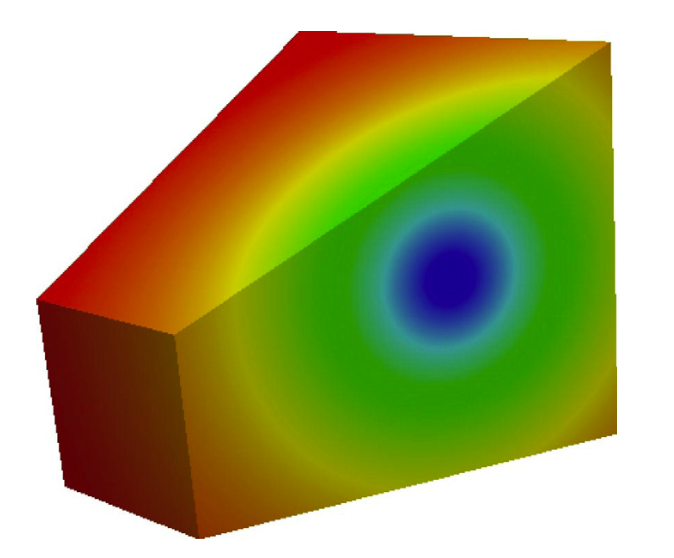
\includegraphics[width=4.2cm]{original-6}    % The printed column width is 8.4 cm.
    \caption{Truncated pyramid geometry. The colours represent the magnitude of the exact solution $\phi$.} 
    \label{fig:original-6}
\end{center}
\end{figure}

The carried out convergence analysis is shown in Fig.~\ref{fig:original-7}. Even if the domain in not the simple sphere, we obtained a first order error for $\phi$. In the case of the potential normal derivative we observe the occurrence of an error plateaux for the $L_\infty$
norm in corresponding to the last refinement level considered. A possible cause can be assessed through an inspection of the local $\frac{\partial\phi}{\partial n}$ error distribution presented in Fig.~\ref{fig:original-8}. As can be seen, the maximum error occurs in correspondence with the edge characterised by the sharpest angle of the figure.

\begin{figure*}
\begin{center}
    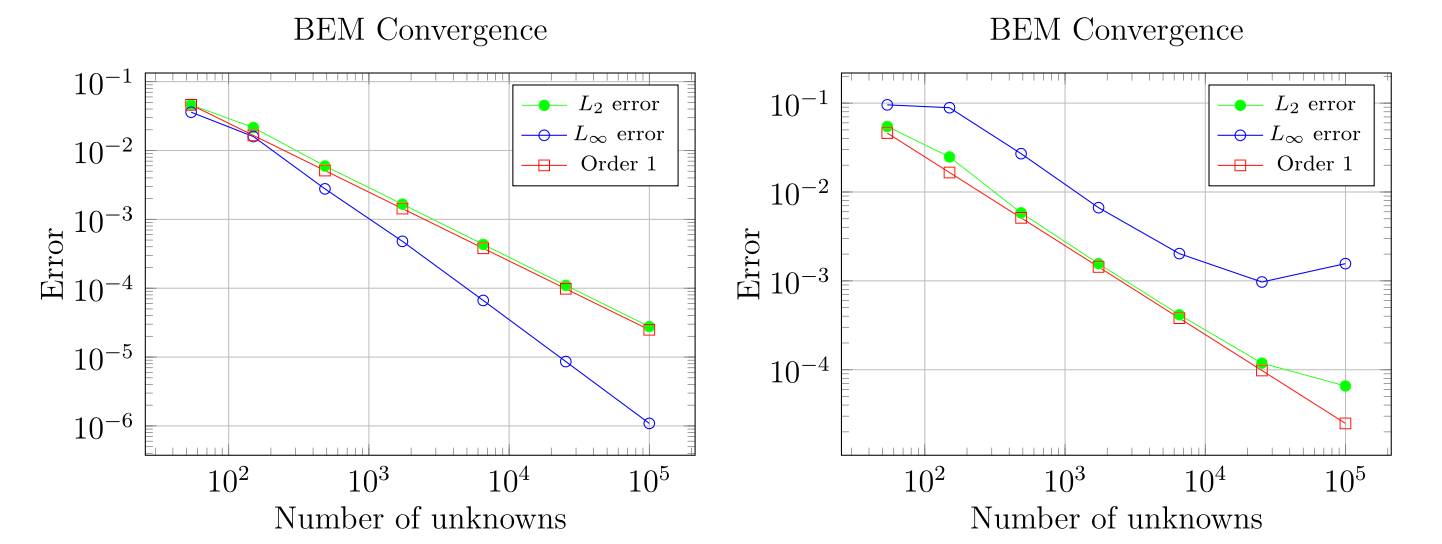
\includegraphics[width=14cm]{original-7}    % The printed column width is 8.4 cm.
    \caption{Convergence analysis for the error in a mixed Dirichlet-Neumann problem using $Q_1$ boundary elements and the truncated pyramid mesh. On the left we plot the analysis for the variable $\phi$, on the right we depict the errors for $\frac{\partial\phi}{\partial n}$.} 
    \label{fig:original-7}
\end{center}
\end{figure*}

\begin{figure}
\begin{center}
    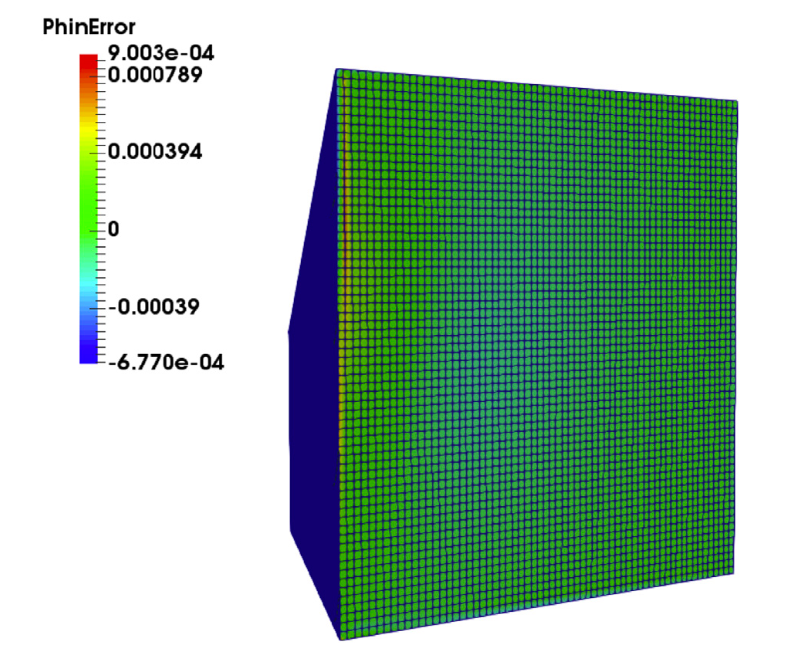
\includegraphics[width=6cm]{original-8}    % The printed column width is 8.4 cm.
    \caption{Error analysis for the potential normal derivative in the truncated pyramid test case.} 
    \label{fig:original-8}
\end{center}
\end{figure}


















%!TEX root = ../main.tex

\section{Parallelisation}
\label{sec:Parallelisation}

At this point, we aim to develop an efficient parallelization strategy to achieve greater computational efficiency. Initially, we analyzed the bottlenecks in the straightforward implementation of BEM, followed by assessing the performance of the parallelization using both strong and weak scaling analysis.

\subsection{Matrix Assembling and Domain decomposition}
\label{sub:matrix_assembling}

Table~\ref{tb:truncated-py} with computational times refers to the truncated pyramid test case on a single CPU. This test case involves using the BEM to evaluate the solver's performance on a geometrically complex domain shaped like the one in Fig.~\ref{fig:original-6}. It requires handling sharp edges and corners with high accuracy, which poses significant computational challenges.

\begin{table}[hb]
\begin{center}
\caption{Profiling on a single CPU.}\label{tb:truncated-py}
\vspace{-0.5em}
\begin{tabular}{ll}
\hline
Function & Time (s) \\
\hline
Assemble cycle & 68.44 \\
Solvetime & 5.741 \\
Post process (Gradient Recovery) $\qquad$ & 0.1645 \\
Total time & 78.6 \\ 
\hline
\end{tabular}
\end{center}
\end{table}

As we can see, matrix assembly is the major part of the overall program computationally demanding, for this reason, it has to be parallelized. We used a collocation scheme to solve the boundary integral formulation. Provided that the whole computational grid is available on each processor, every line of the matrix can be assembled independently. This is because the process of matrix assembling in BEM involves calculating the interactions
between each basis function and each collocation point across the entire domain. Since each row of the system matrix is basically an integral involving a collocation point and all basis functions, and can be computed independently of others, this matrix assembling task is ideal for parallel execution. For this, we utilized MPI to distribute the task of assembling different rows of the matrix to multiple processors. To preserve the parallelisation efficiency, it is mandatory to achieve a proper work balance between different processors.

\begin{figure}
\begin{center}
    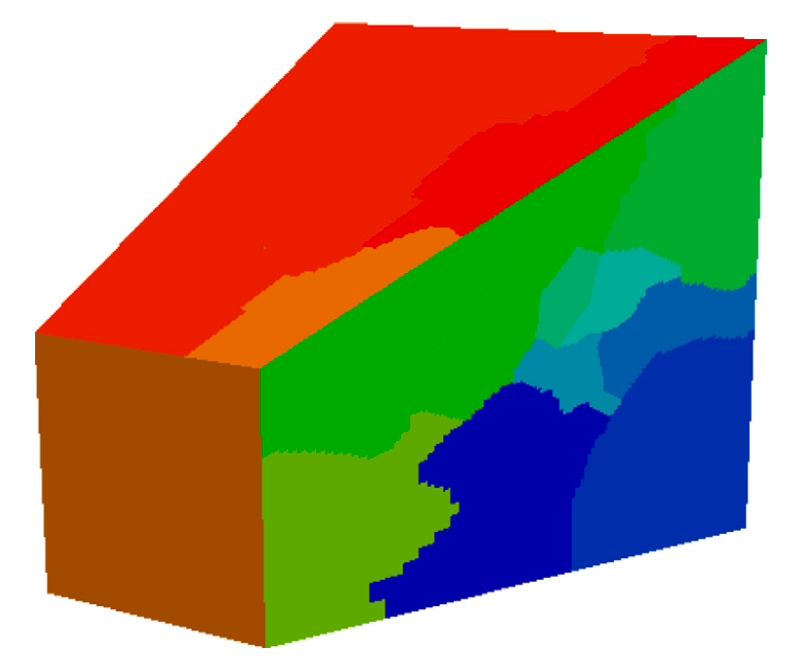
\includegraphics[width=4.2cm]{original-17}    % The printed column width is 8.4 cm.
    \caption{Domain decomposition between 16 different MPI processors.} 
    \label{fig:original-17}
\end{center}
\end{figure}

Fig.~\ref{fig:original-17} indeed represents the domain decomposition between 16 different MPI processors. This non-trivial domain decomposition is due to the local refinement.  It is important to highlight the main difference between BEM and FEM methods, indeed the final matrix in BEM is a smaller but dense matrix, and this is due to the fact that each matrix entry depends on information on the entire boundary of the domain, so every processor still needs access to the full discretisation of the boundary of the geometry, that has not to be confused with the domain decomposition that is related with the
collocation points that every MPI processor has to take into account for a proper workbalance as we mentioned. It could seems that sharing the whole domain to all processor is a bottleneck, but is not, since it is just the boundary domain to be shared, in opposite with the FEM parallelisation method, in which it is mandatory not to share the whole domain. Finally the problem is solved using a parallel implementation of a preconditioned GMRES solver. The preconditioner used is derived from an Incomplete Gauss factorization, which helps reduce the computational load and iteration count necessary for solving.

\subsection{Strong and Weak Scaling}
\label{sub:strong_and_weak_scaling}

The analysis proceeds by evaluating the strong and weak scalability of the previously described problem. We executed a scaling analysis with a total of 40 processors. However, the infiniband network drivers only allow for 16 MPI processors and we will see how this can influence scalability results.

\begin{figure*}
\begin{center}
    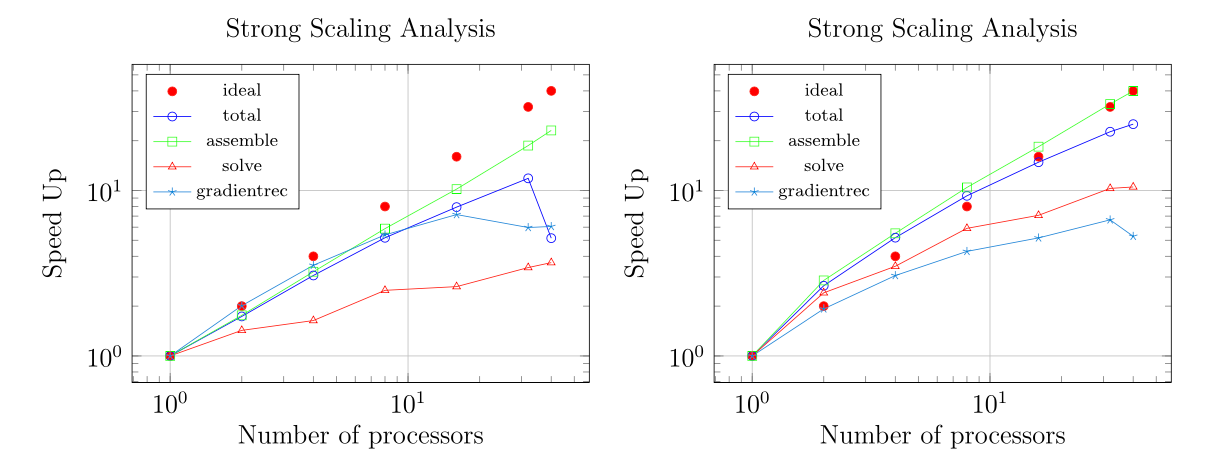
\includegraphics[width=14cm]{original-18}    % The printed column width is 8.4 cm.
    \caption{Strong scalability test. In particular, on the left there is the analysis using 6534 degrees of freedom and on the right the analysis using 25350. In blue with circles we plot the total scalability, in green with squares the performances of the full matrix assembling, in cyan with stars the gradient recovery scalability, and in red with triangles the performance of the linear solver. The red dots represent the ideal speed-up that is of course linear.} 
    \label{fig:original-18}
\end{center}
\end{figure*}

Fig.~\ref{fig:original-18} represents the strong scalability test. As we can see, in the real problem, it is the gradient
recovery and the solve computation that led to a sub-optimal total scalability, and this is even more present in the left graph. This is due to the communication overhead among processors in the
MPI environment because matrix-vector multiplication requires a lot of communication. Notice that the assembly is almost optimal because it doesn’t require any communication. The super optimality in the right test is due to cache resources. We can see an increase in the total performance when considering more degrees of freedom, and this is reasonable because it implies that every MPI processor has to take into account more inner computation,
leading to the communication time becoming less impactful. However, at the same time using more processors involves more communication among them. We could also notice that even
if the solve speed-up is really below the ideal, this doesn’t affect so much the overall performance, and this is due to the relative importance of the assembling versus solving cycles.

Moving forward with the weak scaling, we report the weak scalability analysis in Fig.~\ref{fig:original-20}.

\begin{figure}[htp]
\begin{center}
    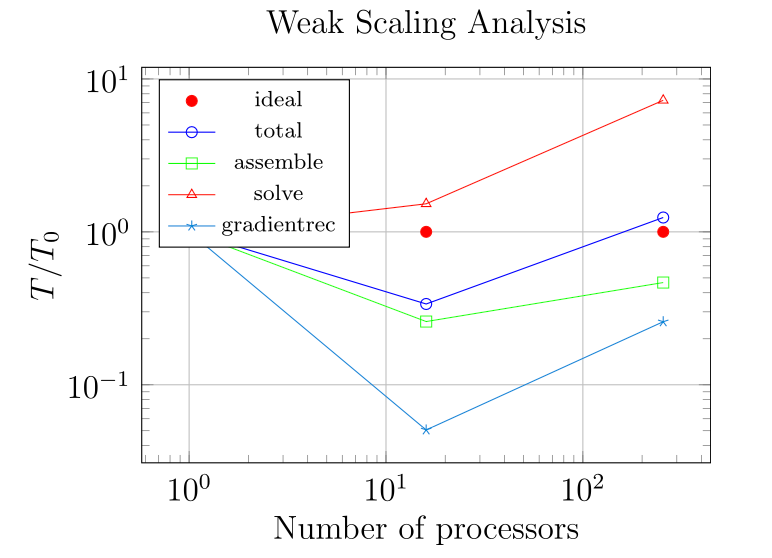
\includegraphics[width=7cm]{original-20}    % The printed column width is 8.4 cm.
    \caption{Weak scalability test. In blue with circles we plot the total performance, in green with squares the timing ratio of the full matrix assembling, in cyan with stars the gradient recovery performance, and in red with triangles the performance of the linear solver. The red dots represents the ideal timings.} 
    \label{fig:original-20}
\end{center}
\end{figure}

The analysis is carried out using up to 256 MPI processors and 25350 degrees of freedom. In particular, we wanted to ensure that each processor handles approximately the same number of matrix entries, thus maintaining a fixed workload per processor in the scaling analysis. If the workload per processor is fixed, we expect that the execution time should remain constant regardless of the number of processors, and the results highlight the desired output. Indeed, the assembling routine has a superoptimal behavior. This is probably due to the structure of the assembling cycle because each processor has to loop over all the cells $N$ times less. However, if we increase the number of MPI processors to 256, we increase dramatically the computational costs for the linear solver, explaining the suboptimal behavior of the solving phase.
%!TEX root = ../main.tex

\section{Accelerated BEM}
\label{sec:fast}

We now focus on a more efficient BEM solver. Indeed, the cost for the solution of standard BEMs remains quadratic: $O(N^2)$, due to the dense structure of their system matrices. This fact poses limitations on the number of degrees of freedom that can be
considered, both in terms of memory requirements and computational times. Exploiting the
structure of the fundamental solution $G$ to approximate the convolution integrals when two
cells are well separated leads to the well-known Fast Multipole Method (FMM), which reduces the computational cost from $O(N^2)$ to $O(N)$. 

\begin{figure*}[!ht]
\begin{center}
    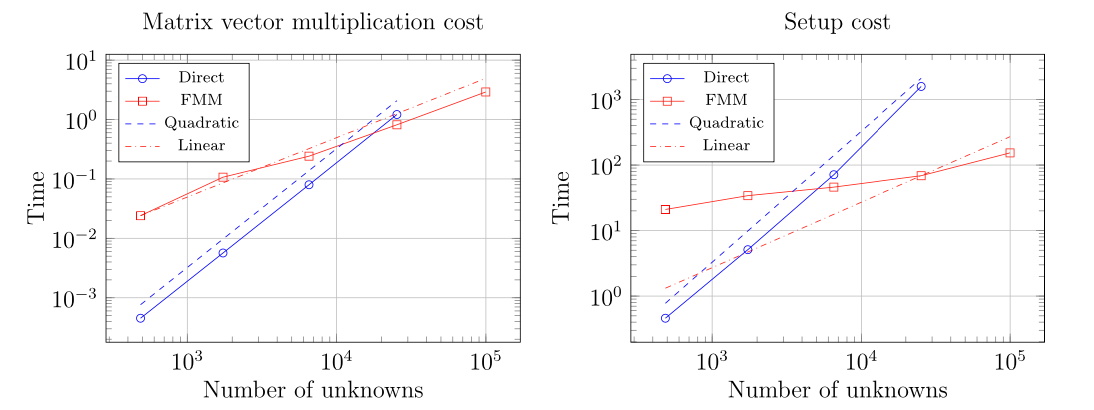
\includegraphics[width=14cm]{original-22}    % The printed column width is 8.4 cm.
    \caption{Computational cost comparison between BEM and BEM-FMM. The figure on the left reports a comparison of a single matrix vector multiplication, the one on the right reports a comparison of the setting time needed by the method.} 
    \label{fig:original-22}
\end{center}
\end{figure*}

\subsection{Fast Multipole Method}
\label{sub:fast_multipole_method}

First, we briefly introduce the FMM. The algorithm was originally derived for $N$-body
problems and it takes into account $N$ evaluation points (nodes) and $M$ charges (sources) that
are distinct in space. $N$-body problems are typical in electromagnetic applications where
one is interested in computing the force exerted by the charges at the evaluation points. The computation is based upon pairwise evaluations of electromagnetic
potential which coincide with the Green functions considered in this paper. This results in the
evaluation of $NM$ source-target distances. If the source and target points coincide, we
recover the quadratic cost $O(N^2)$. The Fast Multipole Method is based on the consideration
that an harmonic expansion of the electromagnetic potential of a single charge allows the
separation into distinct factors of the effects of the source and evaluation point respectively.
In principle, these factors can be computed separately only once for each source and node
point, leading to a $O(N)$ computational cost. In practice, the harmonic series converges only
when target and node points are well separated. Thus, one important building block of the
FMM is a hierarchical space subdivision that is used to decide whether harmonic
expansions or direct potential evaluations are to be used. Observing that the
electromagnetic potential of a single charge coincides with the free space Green functions
employed in most BEM discretisations, it is possible to modify the FMM algorithm and
integrate it into a BEM solver so that we recover the $N$-Body problem. It’s important to
highlight that even if we are considering a complex geometry case and local refinement, we
are still in the FMM framework. This just led to an algorithm that carefully manages the cells in
order to maintain the harmonic convergence, and this is also valid for the weakly singular integrals coming from the boundary integral formulation: we have to deal with specific quadrature formulas, so in such conditions it is not possible to exploit an external FMM library without implementing massive changes while the $\pi$-\texttt{BEM} adapted these characteristics. We
proceed with a comparison between our FMM-BEM and the direct BEM formulation in terms of accuracy and computational costs.

Fig.~\ref{fig:original-22} represents the computational cost comparison between BEM and BEM-FMM. On
the left, it reports a comparison of a single matrix-vector multiplication, and on the right, the setting time needed by the method. As we can see, we obtain the expected linear behavior even if
the break-even point is roughly located at $10^4$ unknowns. For what concerns the accuracy,
the FMM algorithm introduces an error associated with the truncation of the harmonic series
expansions of the type
\begin{equation*}
e_{_\text{FMM}}\leq C \left| \frac{r}{z}  \right|^{p+1}\leq \left( \frac{1}{2}  \right)^{p+1},
\end{equation*}

where $r$ represents the radius of the sphere used to generate the Multipole expansion, $z$ is
the minimum distance between such a sphere and the evaluation node, and $p$ is the truncation order of the Multipole expansion. In FMM algorithm the expansion is only used for sources and nodes lying in \emph{well separated} boxes.

In Fig.~\ref{fig:original-23} we report the convergence rate of the FMM to the direct matrix vector product evaluation (left plot) and to the standard BEM solution (right plot). Also in this case we can see the expected behavior, as the $L_2$ and $L_\infty$ errors lead below the exponential error bounds.

\subsection{FMM Hybrid Parallelisation}
\label{sub:fmm_hybrid_parallelisation}

Here we challenge the parallelisation of FMM-BEM. A key-step is the computation of the so called \emph{Locally Essential Tree} (LET) that drives the overall MPI communication in an optimal way, but one of our implementation choices is the automatic domain decomposition which doesn’t guarantee the construction of such hierarchical tree. This led us to use a multithreaded parallelisation, also due to the
replicated data structures among nodes. We restrict the
distributed memory parallelisation to the most demanding phases of the algorithm by enforcing that the number of threads and the number of MPI processes is kept well balanced at all times. 

Before going on is necessary an overview on the key step of the Fast Multipole Algorithm: in essence, the so-called hierarchical tree is built, which is the name given to the subdivision of the domain into cells that are in turn divided into smaller cells (higher levels).
The last level is represented by the leaves. The algorithm efficiently leverages the multipole expansion at various levels following an ascending phase and a descending phase in which it traverses the levels of the tree. 

\begin{figure*}[!htp]
\begin{center}
    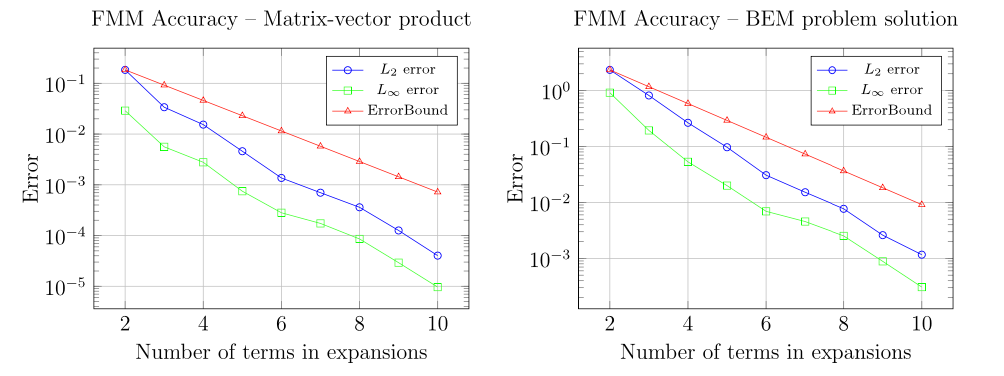
\includegraphics[width=14cm]{original-23}    % The printed column width is 8.4 cm.
    \caption{Convergence analysis for the Multiple expansion using 486 unknowns on the pyramid test case. On the left we report the error of a single matrix vector multiplication, on the right we plot the error on the overall solution.} 
    \label{fig:original-23}
\end{center}
\end{figure*}

One of the most important parameters in the FMM is the number $B$ of evaluation points allowed per leaf of the tree. We want to get some insights on the better tuning of the parameter $B$ to ease the overall computational time of the BEM-FMM algorithm. Greengard and Gropp (see \ref{grop}) derived a simplified analysis of the computational costs to recover an optimal size for the block. We repeat such simplified analysis for the presented FMM in the hybrid shared (TBB) distributed (MPI) memory framework. By defining
\begin{equation*}
\begin{aligned}
N & = \text{number of unknowns}, \\
B & = \text{number of unknowns in a leaf}, \\
p & = \text{number of MPI processors}, \\
t & = \text{number of TBB threads}, 
\end{aligned}
\end{equation*}
the FMM can be sketched as:
\begin{equation}
\label{eq:sum-TFMM}
T_{\text{FMM}} = T_{\text{ascending}} + T_{\text{descending}} + T_{\text{direct}} + T_{\text{comm}},
\end{equation}

where $T_{\text{ascending}}$ represents the time needed by the ascending phase, $T_{\text{descending}}$ is the time needed by the descending phase, $T_{\text{direct}}$ represents the time needed by the short range interactions, while $T_{\text{comm}}$ is the time required by the parallel communications or
synchronisations. If we expand all the terms in Eq.~\eqref{eq:sum-TFMM} we obtain
\begin{equation}
\label{eq:complex-T-formula}
\begin{aligned}
T_{\text{FMM}} =& K_1 \frac{N}{t}+K_2\log_8\left( \frac{N}{B}  \right)\frac{N}{Bt}+K_3\log_8  \left( \frac{N}{B}  \right)\frac{N}{Btp} \\
& +K_4\frac{N}{tp}+K_5\frac{NB}{tp} + e(B,p,t),
\end{aligned}
\end{equation}

where $K_1, K_2, K_3, K_4, K_5$ are experimentally constants that depend on the characteristic of the underlying computational architecture considered, and the function $e$ represents the communication and synchronization cost. Eventually, it can be
easily recover the optimal $B$ by computing the partial derivative of $T_{\text{FMM}}$ with respect to $B$:
\begin{equation}
B_{\text{opt}}=\sqrt{\frac{(K_2+K_3/p)\log_8(N)}{K_5/p} }.
\end{equation}

Fig.~\ref{fig:original-24} represents analysis of the time needed by the overall FMM, considering 1 MPI processor and up to 10 threads per processor, with the number of evaluation nodes per block $B$ varying from 20 to 140. In blue are reported theoretical results using Eq.~\eqref{eq:complex-T-formula}, in green we can see the experimental results. That drastic loss of performance we see is due to the cache-misses. The result is promising since we get that $B_{\text{opt}}=52.5440911254$.

\begin{figure}[!htp]
\begin{center}
    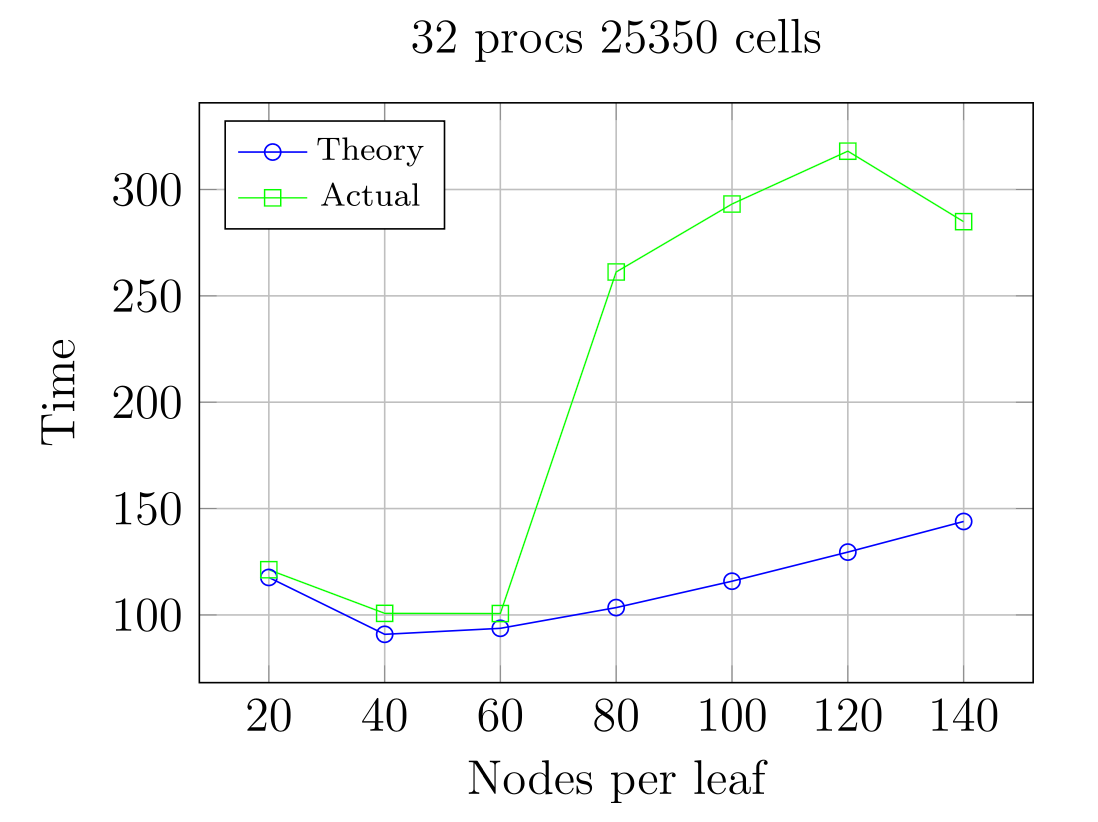
\includegraphics[width=8cm]{original-24}    % The printed column width is 8.4 cm.
    \caption{Analysis of the time needed by the overall FMM.} 
    \label{fig:original-24}
\end{center}
\end{figure}

So for the further analysis we are considering $B$ equal to 60. We highlight that $B_{\text{opt}}$ depends on the number of MPI processor. However, since our FMM is mostly shared memory parallelised, we are not interested in requiring many MPI processors, thus $B = 60$ is a good choice for the scaling analysis.

\subsection{FMM Scaling}
\label{sub:fmm_scaling}

\begin{figure}[!htp]
\begin{center}
    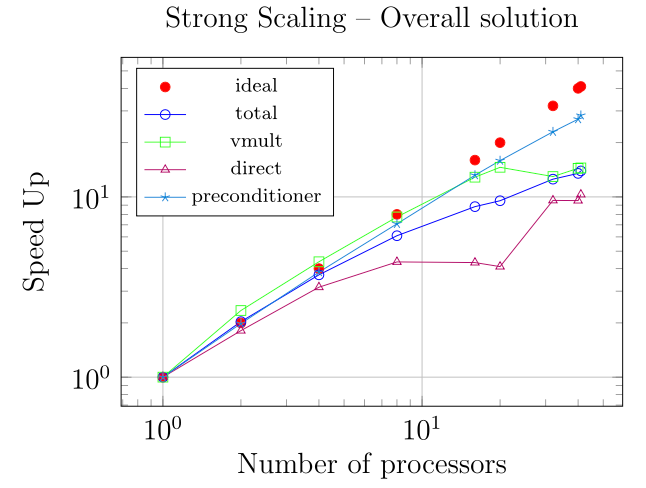
\includegraphics[width=7cm]{original-25-1} \\
    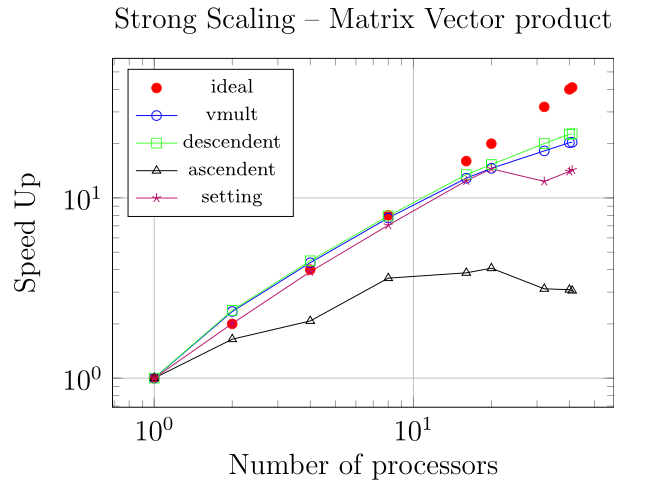
\includegraphics[width=7cm]{original-25-2} % The printed column width is 8.4 cm.
    \caption{Strong Scalability test using 98306 degrees of freedom.} 
    \label{fig:original-25}
\end{center}
\end{figure}

The strong scaling of BEM-FMM algorithm is run
with hybrid TBB-MPI parallelisation up to 2 nodes, each node is composed by two 10 cores, as the previous ones. The top of Fig.~\ref{fig:original-25} represents the strong scaling analysis of the overall algorithm while the bottom illustrates the scalability concerning a single matrix vector multiplication. These plots highlight the scalability issue for short range interactions, and the matrix vector products. Part of the performance loss is induced by the augmented number of iterations needed by the iterative solver when MPI is involved, as suggested by the bottom plot. That plot shows how our
preconditioner is not optimal with rispect to the number of MPI processes. We highlight how the trade-off between computational efficiency and memory is still being studied for a better implementation of the FMM-BEM algorithm, even though we believe the main improvement should come from a better preconditioner.









%!TEX root = ../main.tex

\section{Conclusions}
\label{sec:Conclusions}

In this work, after briefly introducing the history and the main advantages of the Boundary Element Method, we first analysed the scheme in all its theoretical features. Then we presented two test case solved with the $\pi$-\texttt{BEM} library, we faced parallelisation challenges and we showed how a fast hybrid implementation can be derived.


%================================================================

%
\section{Introduction}
This document is a template for \LaTeXe. If you are reading a paper or
PDF version of this document, please download the electronic file
\texttt{ifacconf.tex}. You will also need the class file
\texttt{ifacconf.cls}. Both files are available on the IFAC web site.

Please stick to the format defined by the \texttt{ifacconf} class, and
do not change the margins or the general layout of the paper. It
is especially important that you do not put any running header/footer
or page number in the submitted paper.\footnote{
This is the default for the provided class file.}
Use \emph{italics} for emphasis; do not underline.

Page limits may vary from conference to conference. Please observe the 
page limits of the event for which your paper is intended.


\section{Procedure for Paper Submission}

Next we see a few subsections.

\subsection{Review Stage}

For submission guidelines, follow instructions on paper submission
system as well as the event website.

Note that conferences impose strict page limits, so it will be better
for you to prepare your initial submission in the camera ready layout
so that you will have a good estimate for the paper
length. Additionally, the effort required for final submission will be
minimal.

\subsection{Equations}

Some words might be appropriate describing equation~(\ref{eq:sample}), if 
we had but time and space enough. 

\begin{equation} \label{eq:sample}
%{{\partial F}\over {\partial t}} = D{{\partial^2 F}\over {\partial x^2}}.
\end{equation}

See \cite{Abl:56}, \cite{AbTaRu:54}, \cite{Keo:58} and \cite{Pow:85}.

\subsubsection{Example.} This equation goes far beyond the
celebrated theorem ascribed to the great Pythagoras by his followers.

\begin{thm}   % use the thm environment for theorems
The square of the length of the hypotenuse of a right triangle equals
the sum of the squares of the lengths of the other two sides.
\end{thm}

\begin{pf}    % and the pf environment for proofs
The square of the length of the hypotenuse of a right triangle equals the sum of the squares 
of the lengths of the other two sides.
\end{pf}

%% There are a number of predefined theorem-like environments in
%% ifacconf.cls:
%%
%% \begin{thm} ... \end{thm}            % Theorem
%% \begin{lem} ... \end{lem}            % Lemma
%% \begin{claim} ... \end{claim}        % Claim
%% \begin{conj} ... \end{conj}          % Conjecture
%% \begin{cor} ... \end{cor}            % Corollary
%% \begin{fact} ... \end{fact}          % Fact
%% \begin{hypo} ... \end{hypo}          % Hypothesis
%% \begin{prop} ... \end{prop}          % Proposition
%% \begin{crit} ... \end{crit}          % Criterion

Of course LaTeX manages equations through built-in macros. You may
wish to use the \texttt{amstex} package for enhanced math
capabilities.

\subsection{Figures}

To insert figures, use the \texttt{graphicx} package. Although other
graphics packages can also be used, \texttt{graphicx} is simpler to
use. See  Fig.~\ref{fig:bifurcation} for an example.

\begin{figure}
\begin{center}
\includegraphics[width=8.4cm]{bifurcation}    % The printed column width is 8.4 cm.
\caption{Bifurcation: Plot of local maxima of $x$ with damping $a$ decreasing} 
\label{fig:bifurcation}
\end{center}
\end{figure}

Figures must be centered, and have a caption at the bottom. 

\subsection{Tables}
Tables must be centered and have a caption above them, numbered with
Arabic numerals. See table~\ref{tb:margins} for an example.

\begin{table}[hb]
\begin{center}
\caption{Margin settings}\label{tb:margins}
\begin{tabular}{cccc}
Page & Top & Bottom & Left/Right \\\hline
First & 3.5 & 2.5 & 1.5 \\
Rest & 2.5 & 2.5 & 1.5 \\ \hline
\end{tabular}
\end{center}
\end{table}

\subsection{Final Stage}

Authors are expected to mind the margins diligently.  Papers need to
be stamped with event data and paginated for inclusion in the
proceedings. If your manuscript bleeds into margins, you will be
required to resubmit and delay the proceedings preparation in the
process.

\subsubsection{Page margins.} See table~\ref{tb:margins} for the
page margins specification. All dimensions are in \emph{centimeters}.


\subsection{PDF Creation}

All fonts must be embedded/subsetted in the PDF file. Use one of the
following tools to produce a good quality PDF file:

\subsubsection{PDFLaTeX} is a special version of LaTeX by Han The
Thanh which produces PDF output directly using Type-1 fonts instead of
the standard \texttt{dvi} file. It accepts figures in JPEG, PNG, and PDF
formats, but not PostScript. Encapsulated PostScript figures can be
converted to PDF with the \texttt{epstopdf} tool or with Adobe Acrobat
Distiller.

\subsubsection{Generating PDF from PostScript} is the classical way of
producing PDF files from LaTeX. The steps are:

\begin{enumerate}
  \item Produce a \texttt{dvi} file by running \texttt{latex} twice.
  \item Produce a PostScript (\texttt{ps}) file with \texttt{dvips}.
  \item Produce a PDF file with \texttt{ps2pdf} or Adobe Acrobat
  Distiller.
\end{enumerate}

\subsection{Copyright Form}

IFAC will put in place an electronic copyright transfer system in due
course. Please \emph{do not} send copyright forms by mail or fax. More
information on this will be made available on IFAC website.


\section{Units}

Use SI as primary units. Other units may be used as secondary units
(in parentheses). This applies to papers in data storage. For example,
write ``$15\,\mathrm{Gb}/\mathrm{cm}^2$ ($100\,\mathrm{Gb}/\mathrm{in}^2$)''. 
An exception is when
English units are used as identifiers in trade, such as ``3.5 in
disk drive''. Avoid combining SI and other units, such as current in
amperes and magnetic field in oersteds. This often leads to confusion
because equations do not balance dimensionally. If you must use mixed
units, clearly state the units for each quantity in an equation.  The
SI unit for magnetic field strength $\mathbf{H}$ is $\mathrm{A}/\mathrm{m}$. However, if you wish to
use units of $\mathrm{T}$, either refer to magnetic flux density $\mathbf{B}$ or
magnetic field strength symbolized as $\mu_0\,\mathbf{H}$. Use the center dot to
separate compound units, e.g., ``$\mathrm{A} \cdot \mathrm{m}^2$''.

\section{Helpful Hints}

\subsection{Figures and Tables}

Figure axis labels are often a source of confusion. Use words rather
than symbols. As an example, write the quantity ``Magnetization'', or
``Magnetization M'', not just ``M''. Put units in parentheses. Do not
label axes only with units.  For example, write ``Magnetization
($\mathrm{A}/\mathrm{m}$)'' or ``Magnetization ($\mathrm{A} \mathrm{m}^{-1}$)'', not just
 ``$\mathrm{A}/\mathrm{m}$''. Do not
label axes with a ratio of quantities and units. For example, write
``Temperature ($\mathrm{K}$)'', not ``$\mbox{Temperature}/\mathrm{K}$''.

Multipliers can be especially confusing. Write ``Magnetization
($\mathrm{kA}/\mathrm{m}$)'' or ``Magnetization ($10^3 \mathrm{A}/\mathrm{m}$)''. Do not write
``Magnetization $(\mathrm{A}/\mathrm{m}) \times 1000$'' because the reader would not know
whether the axis label means $16000\,\mathrm{A}/\mathrm{m}$ or $0.016\,\mathrm{A}/\mathrm{m}$.

\subsection{References}

Use Harvard style references (see at the end of this document). With
\LaTeX, you can process an external bibliography database 
using \texttt{bibtex},\footnote{In this case you will also need the \texttt{ifacconf.bst}
file, which is part of the \texttt{ifaconf} package.}
or insert it directly into the reference section. Footnotes should be avoided as
far as possible.  Please note that the references at the end of this
document are in the preferred referencing style. Papers that have not
been published should be cited as ``unpublished''.  Capitalize only the
first word in a paper title, except for proper nouns and element
symbols.

\subsection{Abbreviations and Acronyms}

Define abbreviations and acronyms the first time they are used in the
text, even after they have already been defined in the
abstract. Abbreviations such as IFAC, SI, ac, and dc do not have to be
defined. Abbreviations that incorporate periods should not have
spaces: write ``C.N.R.S.'', not ``C. N. R. S.'' Do not use abbreviations
in the title unless they are unavoidable (for example, ``IFAC'' in the
title of this article).

\subsection{Equations}

Number equations consecutively with equation numbers in parentheses
flush with the right margin, as in (\ref{eq:sample}).  To make your equations more
compact, you may use the solidus ($/$), the $\exp$ function, or
appropriate exponents. Use parentheses to avoid ambiguities in
denominators. Punctuate equations when they are part of a sentence, as
in

\begin{equation} \label{eq:sample2}
\begin{array}{ll}
\int_0^{r_2} & F (r, \varphi ) dr d\varphi = [\sigma r_2 / (2 \mu_0 )] \\
& \cdot \int_0^{\inf} exp(-\lambda |z_j - z_i |) \lambda^{-1} J_1 (\lambda  r_2 ) J_0 (\lambda r_i ) d\lambda 
\end{array}
\end{equation}

Be sure that the symbols in your equation have been defined before the
equation appears or immediately following. Italicize symbols ($T$
might refer to temperature, but T is the unit tesla). Refer to
``(\ref{eq:sample})'', not ``Eq. (\ref{eq:sample})'' or ``equation
(\ref{eq:sample})'', except at the beginning of a sentence: ``Equation
(\ref{eq:sample}) is \ldots''.

\subsection{Other Recommendations}

Use one space after periods and colons. Hyphenate complex modifiers:
``zero-field-cooled magnetization''. Avoid dangling participles, such
as, ``Using (1), the potential was calculated'' (it is not clear who or
what used (1)). Write instead: ``The potential was calculated by using
(1)'', or ``Using (1), we calculated the potential''.

A parenthetical statement at the end of a sentence is punctuated
outside of the closing parenthesis (like this). (A parenthetical
sentence is punctuated within the parentheses.) Avoid contractions;
for example, write ``do not'' instead of ``don' t''. The serial comma
is preferred: ``A, B, and C'' instead of ``A, B and C''.


\section{Conclusion}

A conclusion section is not required. Although a conclusion may review
the main points of the paper, do not replicate the abstract as the
conclusion. A conclusion might elaborate on the importance of the work
or suggest applications and extensions.

\begin{ack}
Place acknowledgments here.
\end{ack}


%================================================================

\bibliography{ifacconf}

%\section*{References}

\begin{enumerate}[label={[\arabic*]}]
\item L. C. Evans. \emph{Partial Differential Equations}, volume 19. American Mathematical Society, 1993. \label{Evans}
\item J. T. Katsikadelis. \emph{The Boundary Element Method for Engineers and Scientist}. Academic Press, 2 edition, 2016. \label{Katsi}
\item Y. J. Liu, S. Mukherjee, N. Nishimura, M. Schanz, W. Ye and A. Sutradhar and E. Pan and A. Dumont and A. Frangi and A. Saez. \emph{Recent Advances and Emerging Applications of the Boundary Element Method}. Applied Mechanics Reviews, 64, 2011. \label{Attilio}
\item A. Mola, N. Giuliani, L. Heltai. \emph{$\pi$-\texttt{BEM}: A flexible parallel implementation for adaptive, geometry aware, and high order boundary element methods}. Advances in Engineering Software, 121:39–58, 2018. \label{Mola}
\item L. Greengard, W. D. Gropp. \emph{A parallel version of the fast multipole method}, volume 20. Computers Math. Applic. 7:63-71, 1990. \label{grop}
\end{enumerate}



%================================================================

%\appendix % Each appendix must have a short title.

%\input{tex/A1FundamentalSolution}


%================================================================

\end{document}
